%!TEX root = ../thesis.tex
%*******************************************************************************
%****************************** Fifth Chapter *********************************
%*******************************************************************************

\chapter{A comparative analysis to distinguish β-cell states and investigate shared transcriptional signatures across T2D-related stressors
}
\label{chapter3}
\newpage

\begin{Comment2}
\vspace{3mm}
\label{contr:chapter2}
\hspace{-3mm}
\textbf{Statement of Contributions} \\\\

\end{Comment2}

\clearpage

\section{An integrated atlas of pancreatic islet \( \mathbf{\upbeta} \)-cells across\\various models of \( \mathbf{\upbeta} \)-cell adaptation and decompensation}
\label{sec:int_atlas}
To better understand the mechanisms underlying successful and failed β-cell compensatory responses, we integrated seven scRNA-seq datasets. We included five datasets generated in-house that included broad ranges of increases in β-cell workload (\textbf{Fig. \ref{fig:3-1} A, Supplementary Table \ref{tab3-1}}), defined as insulin demand per β-cell. We further incorporated two previously published datasets to include  additional hyperglycemic models: islets from older \textit{ob/ob} animals, termed \textbf{Severe genetic obesity} \textbf{\cite{chung_endocrine-exocrine_2020}} and islets from mice subjected to partial β-cell ablation by \gls{stz}, termed \textbf{Partial β-cell ablation} \textbf{(Fig. \ref{fig:3-1} A)} \textbf{\cite{sachs_targeted_2020}}.

\vspace{0.5cm}

\begin{figure}[H]
\centering
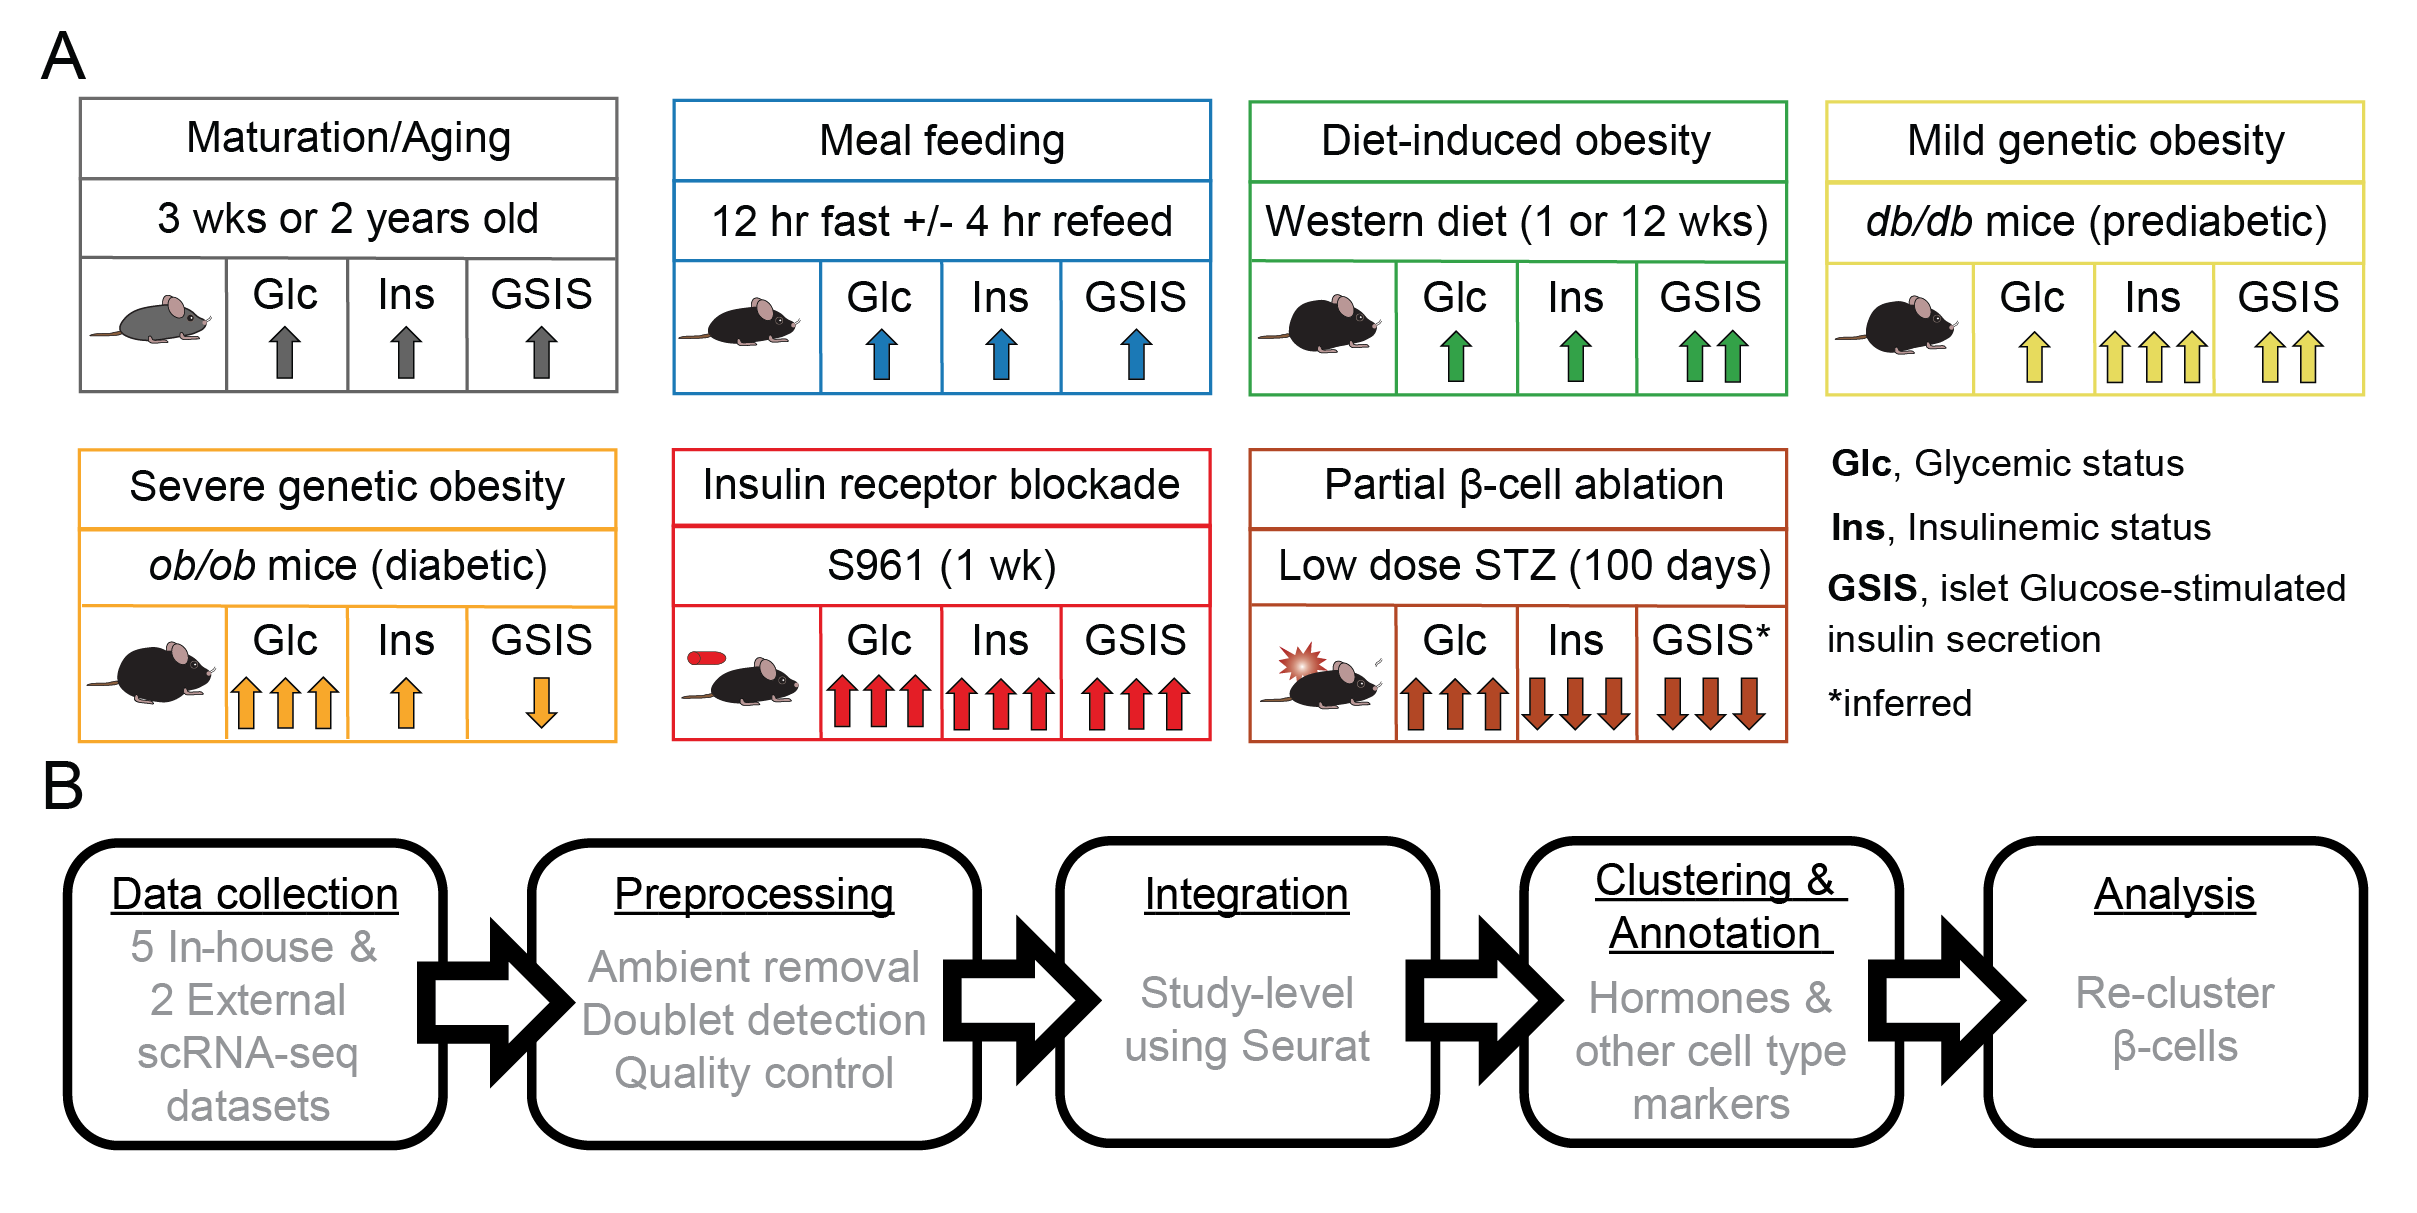
\includegraphics[width=\linewidth]{Chapter5/Fig/F3-1-v2-02.png}
\caption[Workflow to build an integrated atlas to study β-cell transcriptome]{\textbf{Integrated atlas to study β-cell transcriptome in various states that increase workload.} \textbf{(A)} Overview of the various β-cell workload models used in this study. For every model, the effect of the workload on the glycemic, insulinemic and GSIS status of the animals is indicated. The orientation of the arrows indicate the directionality of the response while the number of arrows indicate the intensity. \textbf{(B)} A schematic depicting the workflow for preprocessing, integration, clustering and further downstream analysis.}
\label{fig:3-1}
\end{figure}

%\clearpage

The samples across the seven datasets varied primarily across age (Supplementary Table \ref{tab3-1}). An additional study incorporating islets from 3-week-old (3 wks) or 2-year-old mice, termed \textbf{Maturation/aging}, was used as a reference point for developmental maturity. The same study, along with the data from \textbf{Diet-induced obesity} model were also utilized for the comprehensive analysis of islet-associated immune cells in (\textbf{Chapter \ref{chapter2}}). Out of the seven studies, six of them isolated islets exclusively from male mice, whereas the \textbf{Meal feeding} dataset pooled islets from both male and female mice (Supplementary Table \ref{tab3-1}). Integration of the datasets to be included in the atlas allowed us to account for the various batch-effects arising from sample handling, housing conditions, and mouse strains used. We applied the same pre-processing steps with individual thresholds for every sample across the seven datasets. To enable joint analysis and comparisons of the datasets, we performed data integration in order to create a joint embedding space (\textbf{Fig. \ref{fig:3-1} B}, see \textit{Methods}).\\

% \begin{figure}[H]
% \centering
% 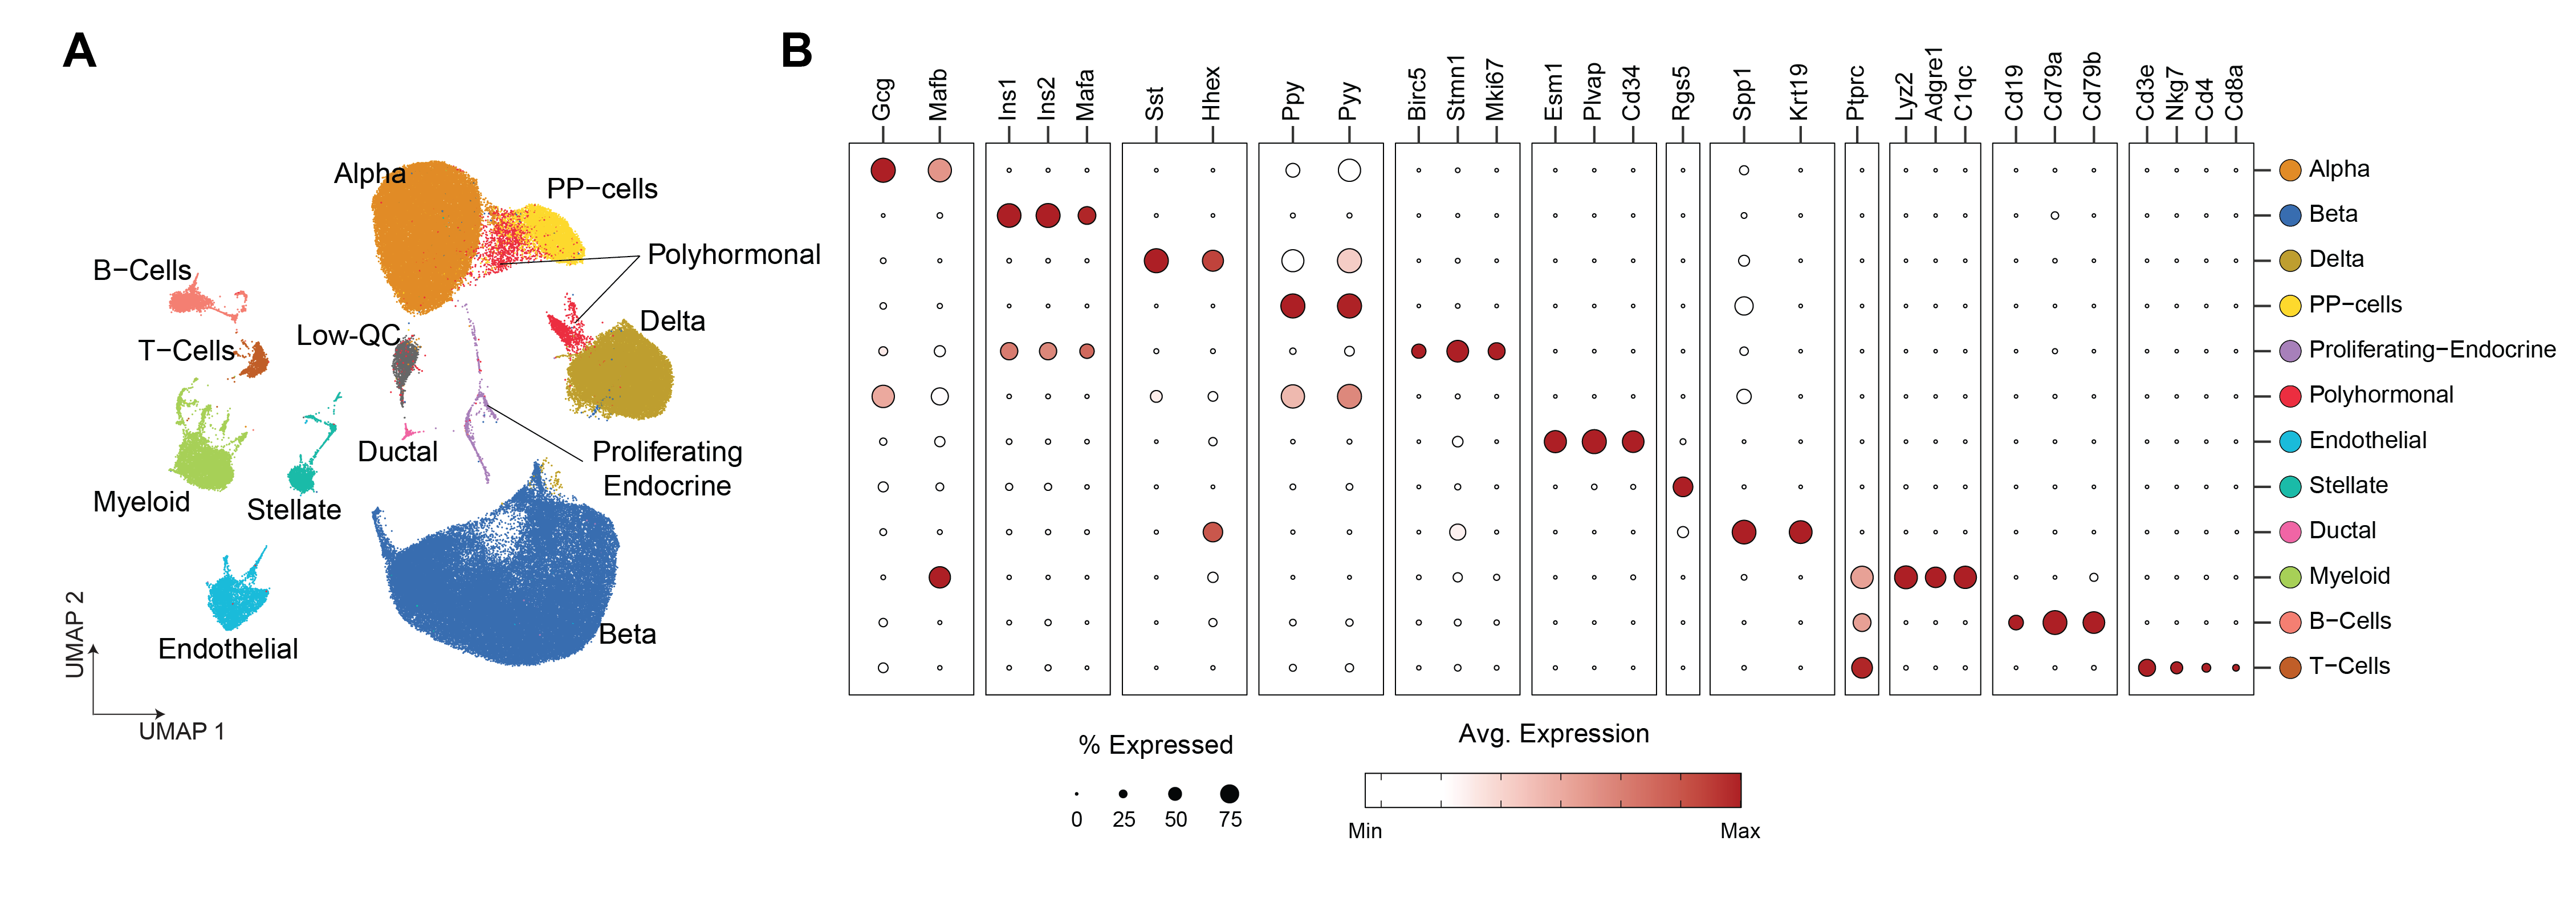
\includegraphics[width=\linewidth]{Chapter5/Fig/F3-2-01.png}
% \caption[fig3-2]{\textbf{Integrated dataset of seven scRNA-seq studies across several models of β-cell decompensation and hyperglycemia.}\\
% \textbf{(A)} UMAP embedding of the integrated dataset depicting celltype annotations based on the expression of known markers. \textbf{(B)} UMAP embedding of the integrated dataset depicting the seven scRNA-seq studies. Datasets are described in Supplementary Table \ref{tab3-1}. \textbf{(C)} Number of cells per sample within each study. \textbf{(D)} Dotplot depicting hallmark markers for the annotated celltypes in panel \textbf{A}. \textbf{E} Number of cells per celltype.}
% \label{fig:3-2}
% \end{figure}
% \clearpage


% \captionof{figure}{\textbf{Integrated dataset of seven scRNA-seq studies across several models of β-cell decompensation and hyperglycemia.} \textbf{(A)} UMAP embedding of the integrated dataset depicting celltype annotations based on the expression of known markers. \textbf{(B)} UMAP embedding of the integrated dataset depicting the seven scRNA-seq studies. Datasets are described in Supplementary Table \ref{tab3-1}. \textbf{(C)} Number of cells per sample within each study. \textbf{(D)} Dotplot depicting hallmark markers for the annotated celltypes in panel \textbf{A}. \textbf{E} Number of cells per celltype.}

%\clearpage

\begin{figure}[H]
\centering
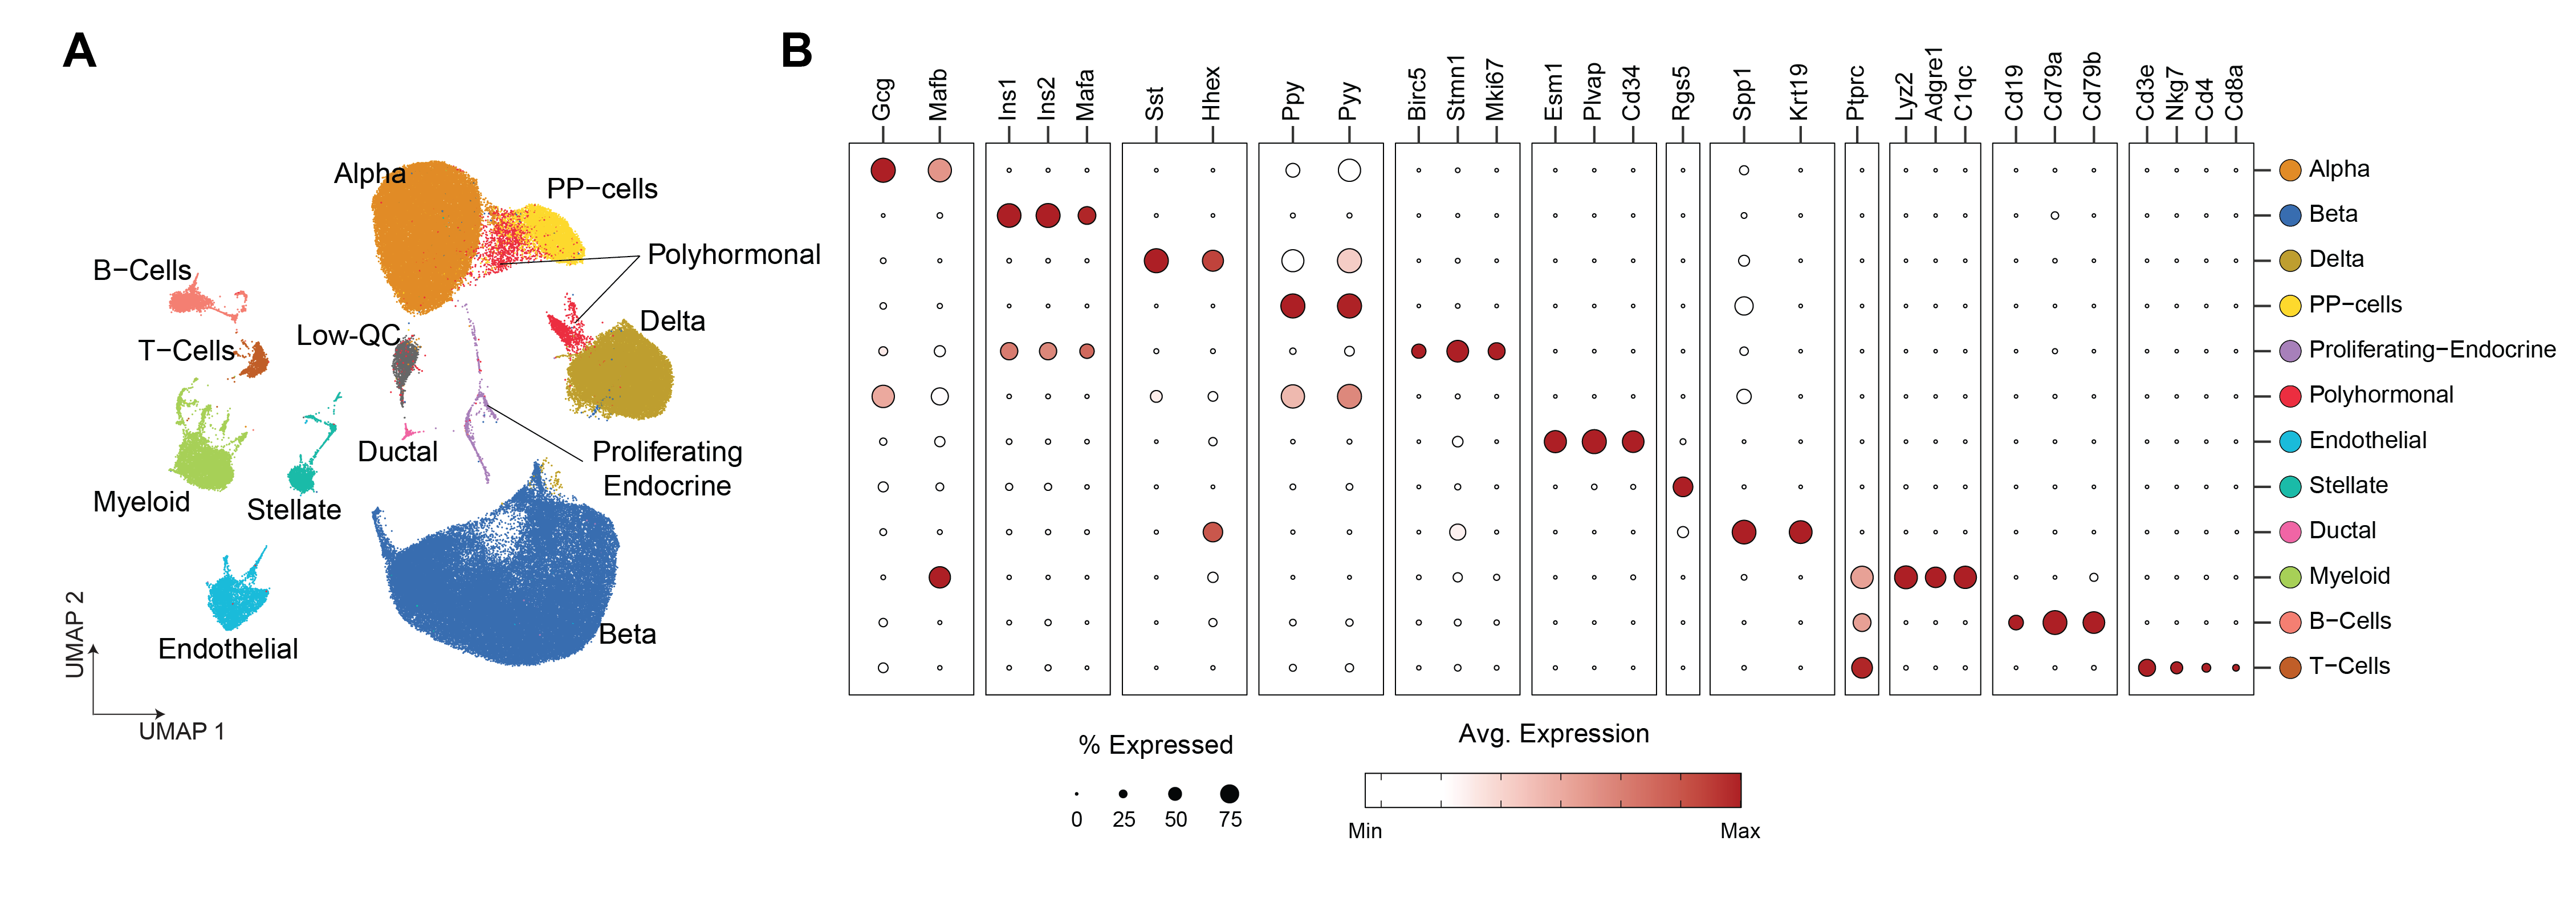
\includegraphics[width=\linewidth]{Chapter5/Fig/F3-2-01.png}
\caption[Annotation of the full integrated dataset using marker genes]{\textbf{Integrated dataset of seven scRNA-seq studies across several models of β-cell decompensation and hyperglycemia.} \textbf{(A)} UMAP embedding of the integrated dataset depicting celltype annotations based on the expression of known markers. \textbf{(B)} UMAP embedding of the integrated dataset depicting the seven scRNA-seq studies. Datasets are described in Supplementary Table \ref{tab3-1}.}
\label{fig:3-2}
\end{figure}

This integrated embedding space showed clear separation into distinct clusters, which corresponded to distinct cell-types that originate from the different datasets \textbf{(Fig. \ref{fig:3-2} A)}. This provided empirical evidence that the previous step of data integration was indeed successful, thereby ensuring optimal trade-off between batch correction and biological conservation on the level of cell-types \textbf{(Fig. \ref{suppl_fig:chp3_study} A)}. The integrated dataset contains 124,191 cells across 16 samples \textbf{(Fig. \ref{suppl_fig:chp3_study} B, Supplementary Table \ref{tab:3-3})}. We manually annotated the four major islet cell-types using the expression of hormone markers: Alpha – \textit{Gcg}, Beta- \textit{Ins1} and \textit{Ins2}, Delta – \textit{Sst} and PP-cells – \textit{Ppy}. Apart from the major hormone secreting cell-types, we also annotated polyhormonal cells expressing more than one hormone marker simultaneously. We identified theses polyhormonal cells by first setting thresholds on hormone expression and then identifying co-expressing cells with any two hormone markers. Based on this, we were able to identify `Alpha-PP’ and `Delta-PP’ as the major polyhormonal contributors. We were also able to identify non-endocrine cell-types such as Endothelial – \textit{Pecam1}, Immune – \textit{Ptprc}, Stellate – \textit{Rgs5} and Ductal – \textit{Krt19} \textbf{(Fig. \ref{fig:3-2} B)}.



\clearpage

\section{Clustering of pseudo-bulk \( \mathbf{\upbeta}\)-cells segregates hyperglycemic\\from normoglycemic samples}
\label{sec:chp3_pseudobulk}

To focus upon transcriptional changes in islet β-cells during compensation and failure, we subset β-cells for further analysis. We subset cells annotated as `Beta' and `Proliferating-Endocrine', performed additional QC to remove polyhormonal cells expressing non-β hormones (\textit{Gcg, Sst, Ppy}), retained the proliferating β-cells, and re-integrated across the seven studies \textbf{(Fig. \ref{fig:3-3} A, Supplementary Table \ref{tab:3-3})}. The re-integration of β-cells was necessary to account for any nested batch effects that might have been persistent across the studies. On the integrated embedding, the β-cells from the healthy controls employing adult mice and the 2 years old mice from Aging/maturation study overlapped with each other, whereas the cells from the experimental samples and the 3 wks old young mice, mapped together and away from the control groups \textbf{(Fig. \ref{suppl_fig:chp3_betastudy})}.\\\\
To provide a stringent assessment of the effectiveness of single-cell integration and to test whether the re-integration of β-cells was adequate for downstream analyses, we performed hierarchical clustering of samples based on the expression profiles of \textit{pseudobulk} β-cells. We aggregated the normalizd expression values of the 3000 \glspl{hvf} across all the experimental samples and the aggregated expression matrix was used to cluster genes into nine modules, grouping genes with similar expression profiles across the samples \textbf{(Fig. \ref{fig:3-3} B)}. Based on these gene modules, hierarchical clustering of the experimental samples separated the hyperglycemic models such as the insulin receptor blockade with S961, obese \textit{ob/ob} animals and partial β-cell ablation with \gls{stz} from their normoglycemic controls. However, these normal controls did not cluster with the healthy controls of the remaining studies likely due to enduring batch effects between the studies. The \textit{dbHet} animals of 6 and 9-weeks old clustered together and away from the \textit{db/db} cohorts, which also clustered together. Similarly, samples with mice fed chow diet for 1 or 12 weeks clustered together and away from the WD-fed counterparts of both time-points. Interestingly, the fasting and feeding samples from the Meal feeding study clustered together \textbf{(Fig. \ref{fig:3-3} B)}, reflecting the minimal effect of the feeding intervention on β-cell workload compared to models that exerted higher workloads on the β-cell.\\

%\clearpage

\begin{figure}[t]
\centering
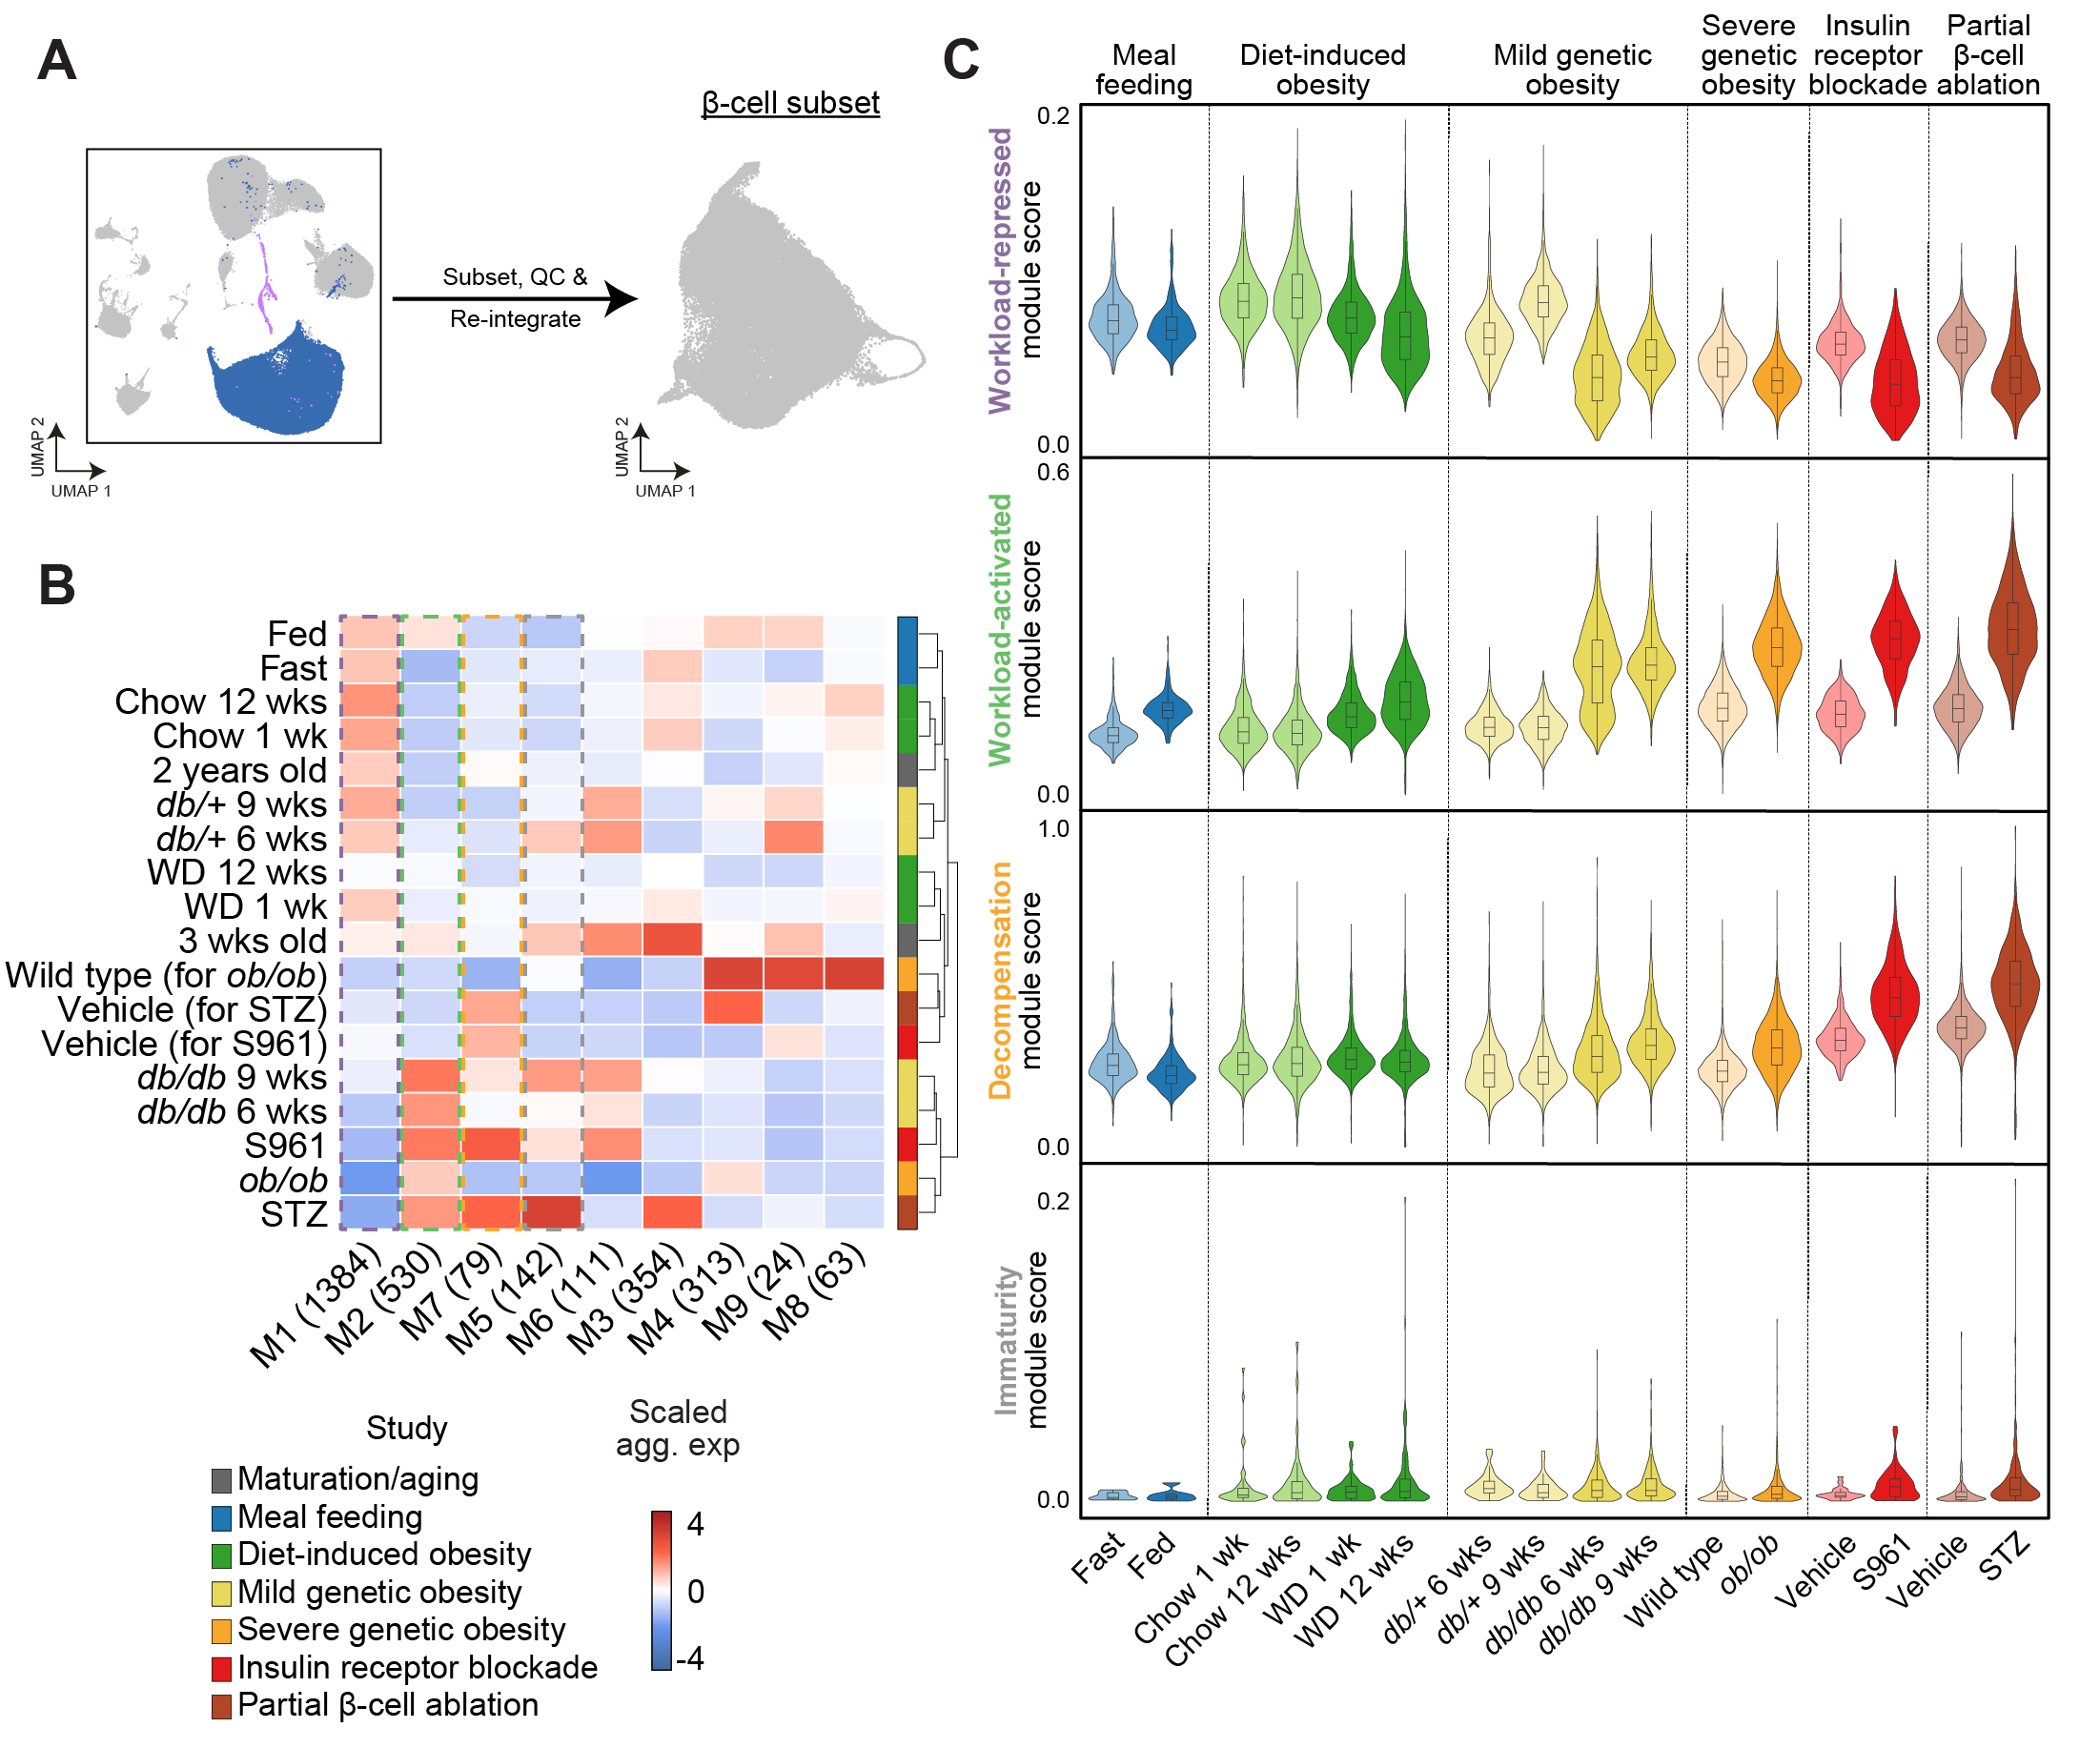
\includegraphics[width=\linewidth]{Chapter5/Fig/F3-3-01.png}
\caption[Hierarchical Clustering of pseudobulk β-cells across the samples]{\textbf{Hierarchical Clustering of pseudobulk β-cells across the samples.} \textbf{(A)} Heatmap depicting the hierarchical clustering of samples from seven studies based on the scaled aggregate expression of pseudobulk β-cells. The number of genes in each of the module is indicated in parantheses. \textbf{(B)} Violin plots depicting gene-set score of β-cells across all the samples from six studies for four modules highlighted in panel \textbf{A}. The Maturation/aging study is not depicted.}
\label{fig:3-3}
\end{figure}

We then performed gene-set scoring on a single-cell level for four modules (\textit{Modules M1,M2,M5} and \textit{M7}) identified from the hierarchical clustering of pseudobulk β-cells across the samples \textbf{(Fig. \ref{fig:3-3} C)}. Module \textit{M1} was repressed by all conditions of increased workload and contained known markers of β-cell function (\textit{Mafa, Slc2a2}) and development (\textit{Neurod1, Pdx1}) as well as ion homeostasis (\textit{Atp2a2, Trpm5}) and was termed as `Workload-repressed module' \textbf{(Fig. \ref{fig:3-3} C, \textit{top row})}. On the other hand, module \textit{M2} was activated in response to increased β-cell workload in models of mild (\textit{db/db}) and severe (\textit{ob/ob}) genetic obesity, insulin receptor blockade (S961) and partial β-cell ablation (\gls{stz}). The expression of this module was also slightly elevated in response to feeding as well as in the young 3 wks old mice. Module-2 associated with genes involved in protein processing in ER (\textit{Calr, Dnajb11, Hspa5}) and translation (\textit{Sec11a/c, Spcs1/2}). Therefore, we termed this module as ‘Workload-activated module’ \textbf{(Fig. \ref{fig:3-3} C, \textit{second row})}. In the MIA \textbf{\cite{hrovatin_delineating_2023}}, the authors identified three gene programs (GPs 2,3 and 4) which showed higher activity in the \textit{db/db + mSTZ} state and contained known diabetes markers or were associated with ER stress Based on the overlap of markers, the `Workload-activated' module identified here and GPs 2,3 and 4 from the MIA likely represent the same gene set with genes upregulated in response to increased β-cell workload. We also identified STZ-specific module \textit{M5}, which is likely similar to GPs 8 and 23 identified in MIA, associated with immaturity. Additionally, this analysis also revealed a ‘decompensatory’ profile (\textit{Module-7}), which characterized the insulin receptor blockade as well as the partial β-cell ablation models (S961+\gls{stz}) \textbf{(Fig. \ref{fig:3-3} C, \textit{third row})}. \hl{This module was comprised of ribosomal genes which were upregulated in response to severe hyperglycemia due to S961 or STZ treatment. <need more characterization>}\\\\
In summary, the hierarchical clustering of pseudobulk β-cells provided further evidence for successful re-integration of β-cells from all experimental samples, distinguishing hyperglycemic models from normoglycemic control samples. In normoglycemic controls, samples from low-to-moderate β-cell workload models and severe hyperglycemic models clustered separately, likely due to enduring batch effects. Furthermore, this analysis identified gene sets associated with increasing β-cell workload and with failure. This revealed that β-cell transcriptional signatures of workload-activated genes and hyperglycemia-repressed genes are similar across models.


\clearpage

%\section{Identification and classification of \( \mathbf{\upbeta} \)-cell subsets}
\section{Characterization of \( \mathbf{\upbeta} \)-cell heterogeneity using subset-\\enriched markers}
Classification of β-cell subsets based on
gene ontology analysis of subset-enriched mRNAs

\label{sec:chp3_betaclustering}
As previously discussed, extensive research has shown that β-cells are heterogeneous and this heterogeneity has been re-capitulated at a single-cell level. Independent analysis of the models used in this meta-analysis study identified distinct subtypes with transcriptomic differences relating to maturity and functional status of these β-cells. However, it is unclear how these subtypes relate to each other across several models of β-cell decompensation and failure. Therefore, in order to understand β-cell heterogeneity in a more unified framework and to understand how changes in β-cell workload and changes in glycemic dysregulation affect their transcriptomes, we classified β-cells into six putative subsets using unsupervised clustering \textbf{(Fig. \ref{fig:3-4} A)}. We then predicted cellular processes active in each cluster using GO and pathway analyses of marker genes associated with each cluster.\\\\
Markes expressed highest in β-1 cells were enriched for GOs and pathways such as `oxidative phosphorylation' and `regulation of insulin secretion', including previously described markers of β-cell maturity such as \textit{Mafa, Slc2a2}  and \textit{Ucn3}, and were therefore termed normal β-cells (\textbf{β-1 Normal}) \textbf{(Fig. \ref{fig:3-4} B,C)}. As expected, the β-1 cluster was enriched in the unchallenged controls of six studies (Meal feeding, Diet-induced obesity, Mild and Severe genetic obesity, Insulin receptor blockade and partial β-cell ablation) as well as in the 2 years old mice from the Aging/maturation model \textbf{(Fig. \ref{fig:3-4} D)}.\\\\
The β-3 cluster was characterized by expression of genes enriched in the GO term `cellular responses to stress' and by markers of immaturity \textbf{(Fig. \ref{fig:3-4} B,C)}. The β-3 cluster was not enriched upon meal feeding compared to fasting control or by WD feeding for 1 or 12 weeks, wherein the proportion of β-3 cells was similar to chow-fed controls. In the Maturation/aging study, the early development stage (3 wks old) also showed an enrichment of the β-3 cluster compared to the aged mice. In models of hyperglycemia, the proportion of the β-3 cluster was strongly expanded in challenged mice compared to their corresponding controls. This enrichment was strongest in the \gls{stz}-treated mice, which had the highest proportion of this cluster among all the other cohorts \textbf{(Fig. \ref{fig:3-4} D)}. This was also evident in the original study, in which the authors identified a β-immature state that becomes abundant in \gls{stz}-treated islets, and shows upregulation of genes involved in ER stress and oxidative phosphorylation. This suggests that β-3 cluster likely resembles β-mSTZ cells from \textbf{\cite{sachs_targeted_2020}} in transcriptional profile. Based on these observations, we termed the β-3 cluster as ‘\textbf{Stress-immature}’, as the immature nature of β-cells in this cluster can likely be attributed to the severe workload of these cells under conditions of severe hyperglycemia (and insulin resistance).\\

\begin{figure}[t]
\centering
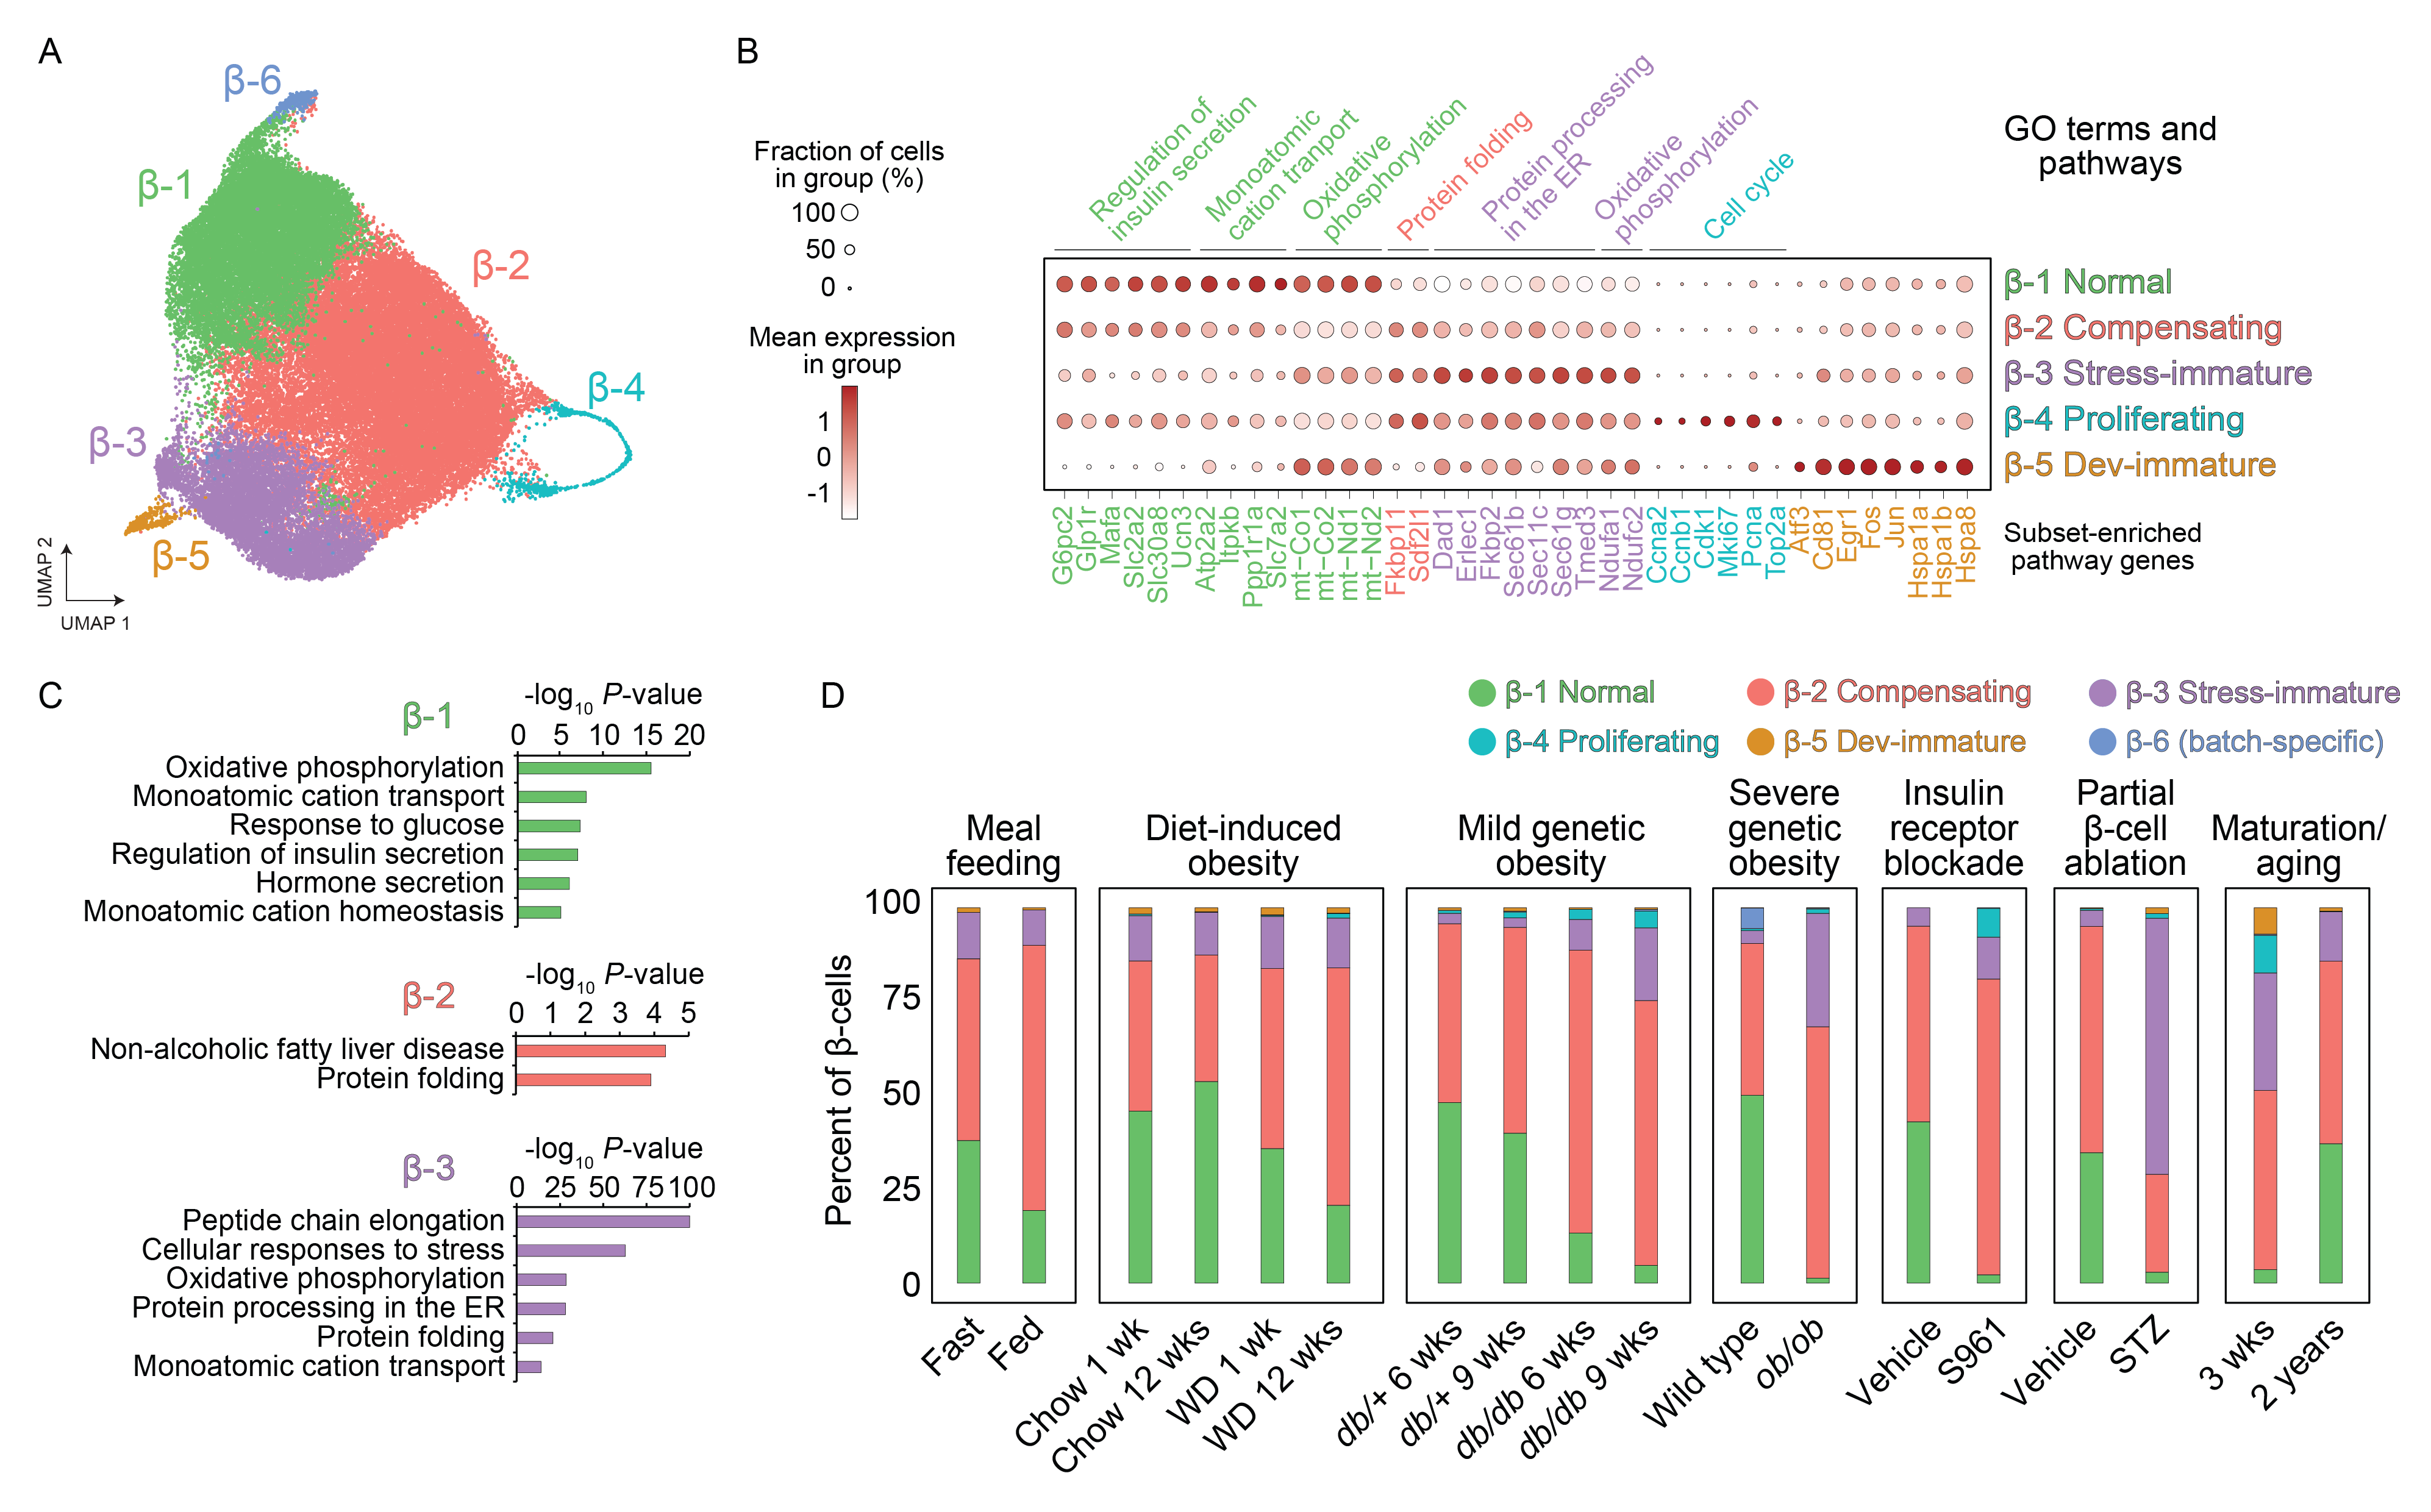
\includegraphics[width=\linewidth]{Chapter5/Fig/F3-1-v2-03.png}
\caption[Characterization of β-cell heterogeneity using subset-
enriched markers]{}
\label{fig:3-4}
\end{figure}

Genes expressed most highly in the β-2 cluster, constituting the largest β-cell subset, were enriched for the GO term `Protein folding' mainly comprising genes encoding ER resident proteins including chaperones and prolyl isomerases \textbf{(Fig. \ref{fig:3-4} B,C)}. The upregulation of ER machinery may signify an adaptive response to maintain ER homeostasis during increased requirements for insulin synthesis and processing during elevated β-cell workload. Genes overexpressed in β-2 cells tended to be expressed at intermediate levels in compared to β-1 or β-3 cells \textbf{(Fig. \ref{fig:3-4} B)}, and therefore β-2 associated genes were not as cluster-specific as genes characterizing β-1 or β-3 subsets. Analysis of the composition of β-2 across the studies showed an almost universal enrichment of this subset with increasing β-cell workload \textbf{(Fig. \ref{fig:3-4} D)}. This included the `Meal feeding’ model, which involved a 4-hour window of feeding or additional fasting on the final day. This likely suggests that the composition shift of β-2 observed in fed animals compared to fasted controls is quite rapid and involves changes in cellular state, as this shift outpaces estimates of β-cell turnover that would be necessary to impact abundances of cellular subtypes. Similar enrichment of these β-2 `Compensating’ cells  were observed in the 1 and 12-week WD fed obese adult animals as well as the 6-week-old and 9-week-old \textit{db/db} mice, which are not yet hyperglycemic. The majority of the islets of the hyperglycemic \textit{ob/ob} mice and the S961-treated mice were composed of the β-2 compensating cells \textbf{(Fig. \ref{fig:3-4} D)}, again indicating the severity of the workload experienced by the β-cells in these models. Overall, the observed composition shifts suggest that increases in β-cell workload gives rise to a state switch from β-1 Normal to β-2 Compensating.\\\\
Apart from the three major β-cell clusters, the unsupervised clustering also identified three minor subsets: β-4 cells expressing genes enriched for the GO terms `cell cycle’ and `DNA metabolic process’ including established markers of β-cell proliferation (\textit{Mki67, Top2a}), which we termed ‘Proliferating’ cells \textbf{(Fig. \ref{fig:3-4} B, Fig. \ref{suppl_fig:chp3_betasubsets} A)}. These cells were enriched in the very young 3 wks old mice as well as the S961-treated animals, as expected \textbf{(Fig. \ref{fig:3-4} D)}. The proliferative nature of β-cells in response to increase in workload has been well documented \textbf{\cite{}}. Interestingly, the 3 wks old mice also exhibited a minor subset expressing well-known markers of β-cell immaturity (e.g. \textit{Cd81}) \textbf{(Fig. \ref{fig:3-4} D)}. Such an expression profile indicates this minor subset is likely developmentally immature β-cells, which is yet to establish a mature identity and is distinct from the stressed β-3 subset wherein the immaturity is the result of the metabolic stress caused by hyperglycemia. Thus, the 3 wks old mice seemed to go along with the enrichment of both, stress-immaturity (β-3) as well as developmental-immaturity (β-5). Finally, β-6 comprised a minor subset, specific to the wild-type control for \textit{ob/ob} mice \textbf{(Fig. \ref{fig:3-4} D, Fig. \ref{suppl_fig:chp3_betasubsets} B,C)}; however, it is unclear what this small subset might represent. Of note, the gene module analysis identified module \textit{M8}, which was highly and specifically expressed in this sample \textbf{(Fig. \ref{fig:3-3} B)}, and the transcriptional profile of \textit{M8} was similar to GP25 in the MIA.\\\\

%\hl{<ERAD and UPR scores>}\\
In summary, unsupervised clustering of β-cells revealed six β-cell subsets which were annotated based on characteristic cellular processes of each of the subsets. We identified a normal β-cell cluster with known markers of maturity and function and a stressed β-cell cluster which depicted markers of stress response as well as immaturity. We additionally identified a small developmentally immature subset which can be distinguished from normal β-cells using previously described markers. Taken together, this likely suggests that β-cell immaturity can be associated with developmental or stress-response processes. The majority of β-cells were comprised of `decompensatory' nature, which showed an universal enrichment in response to increasing β-cell workload. Interestingly, this subset lacked any specific markers unlike β-1 or β-3, possibly suggesting that this subset likely corresponds to a β-cell state. Overall, this analysis revealed the heterogeneous landscape of β-cell transcriptome across several models of β-cell decompensation and hyperglycemia. 

\clearpage

\section{}
\label{sec:chp3_betaPCA}
In the above analyses, we identified three major β-cell subsets (β-1 Normal, β-2 Compensating and β-3 Stress-immature) with characteristic cellular processes and distinct compositional shifts during increasing β-cell workload. However, whether these subsets represent discrete subtypes or continuous states, and relationships between them is unclear. Additionally, as previously stated, since the over-expressed genes in the β-2 Compensating subset were not cluster-specific, compared to the β-1 or β-3 subsets, we hypothesized that the compensating state might be better represented by a continuous feature that distinguishes normal and compensating cells along a continuum. Therefore, to further assess the subset annotations of islet β-cells and their compositional shifts in response to increased workload in hyperglycaemic and insulin-resistant models, we utilized \gls{pca} of the re-integrated β-subset.\\


\begin{wrapfigure}{r}{0.5\textwidth}
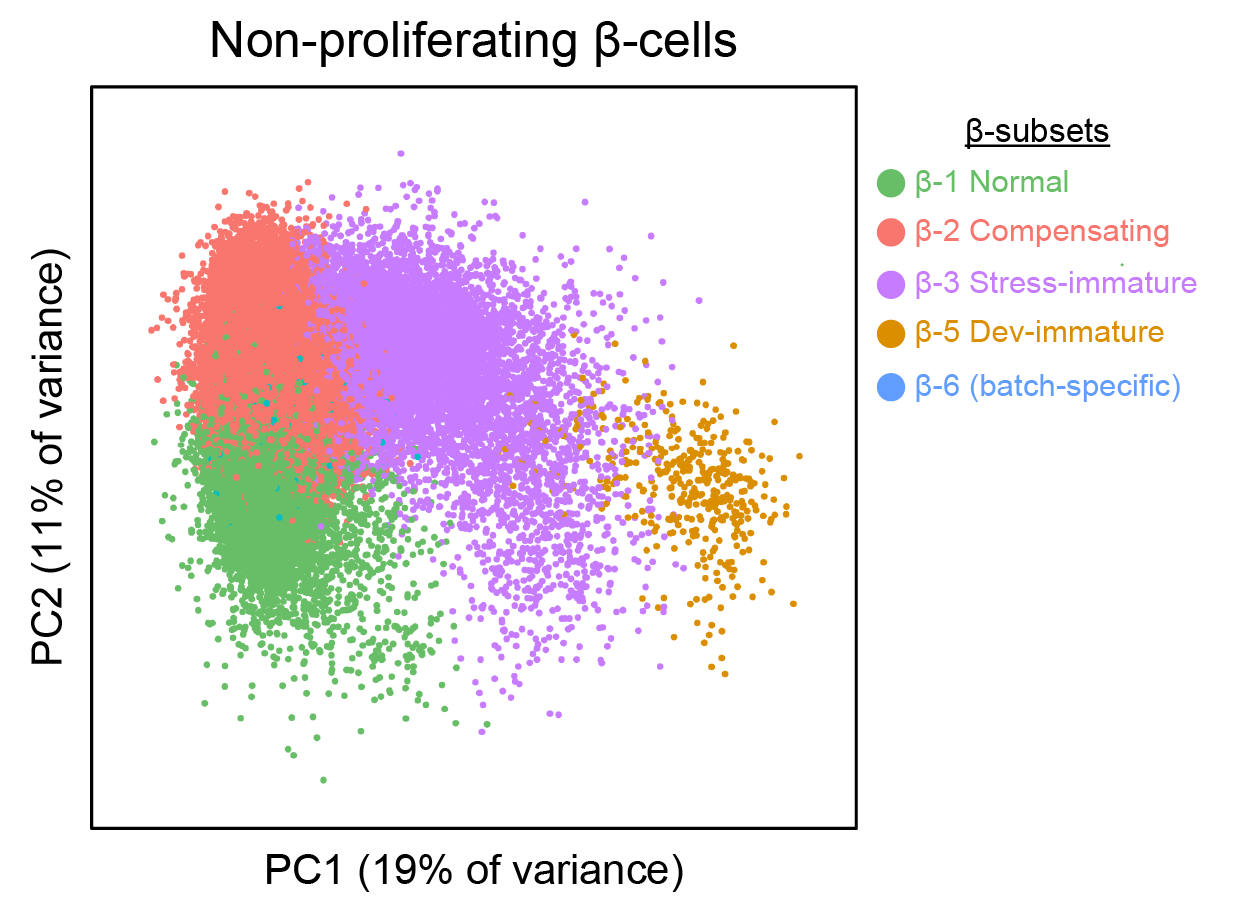
\includegraphics[width=8cm]{Chapter5/Fig/F3-6-01.png}
\caption[PCA of Non-proliferating β-cell subsets]{Principal Component Analysis (\gls{pca}) of non-proliferating β-cells grouped by β-cell subsets across the first two \glspl{pc} (\gls{pc}1 and \gls{pc}2). The percentage of variance explained by each of the two \glspl{pc} are depicted in parentheses.}
\label{fig:3-5}
\end{wrapfigure}


In theory, each principal component (\gls{pc}) represents an axis in a high-dimensional space that captures the largest amount of variation in the data. Thus, the first \gls{pc} is such that it maximizes this variance, the second \gls{pc} captures most of the remaining amount of variation and is orthogonal to the first \gls{pc}. In this way, the top \glspl{pc} are supposed to capture the most dominant factors of heterogeneity in the dataset, In the context of scRNA-seq, it is widely assumed that biological processes affect multiple genes in a coordinated manner whereas random or biological noise would affect each gene independently. %\st{Therefore, the earlier PCs are more likely represent the biological heterogeneity whereas the technical variability would be attributed with later PCs.}
Therefore, it is common practice in scRNA-seq to make use of earlier and top PCs in downstream analysis. This is a simple, highly-effective and widely used strategy in several fields.\\\\

We recomputed the \glspl{pc} for all the non-proliferating β-cells in our re-integrated subset. In our analysis, the first two \glspl{pc} (\gls{pc}1 and \gls{pc}2) were able to distinguish the three major β-cell subsets \textbf{(Fig. \ref{fig:3-5})}. Across the 3000 HVFs, \gls{pc}1 accounted for 19\% of the variance \textbf{(Fig. \ref{fig:3-5})} and corresponded with β-cell maturation state \textbf{(Fig. \ref{fig:3-6}, Fig. \ref{suppl_fig:chp3_pc1})}. This was evident from a histogram plot depicting cell densities along PC1 weights along with which the cells were ordered. Traversing along this `ranked axis’,we observed  that the higher density was accounted by the β-3 Stress-immature subset \textbf{(Fig. \ref{fig:3-6} A)} and β-5 Dev-immature subset \textbf{(Fig. \ref{suppl_fig:chp3_pc1} A)} and thereby distinguishing them from β-1 Normal or β-2 Compensating subsets.


\begin{figure}[H]
\centering
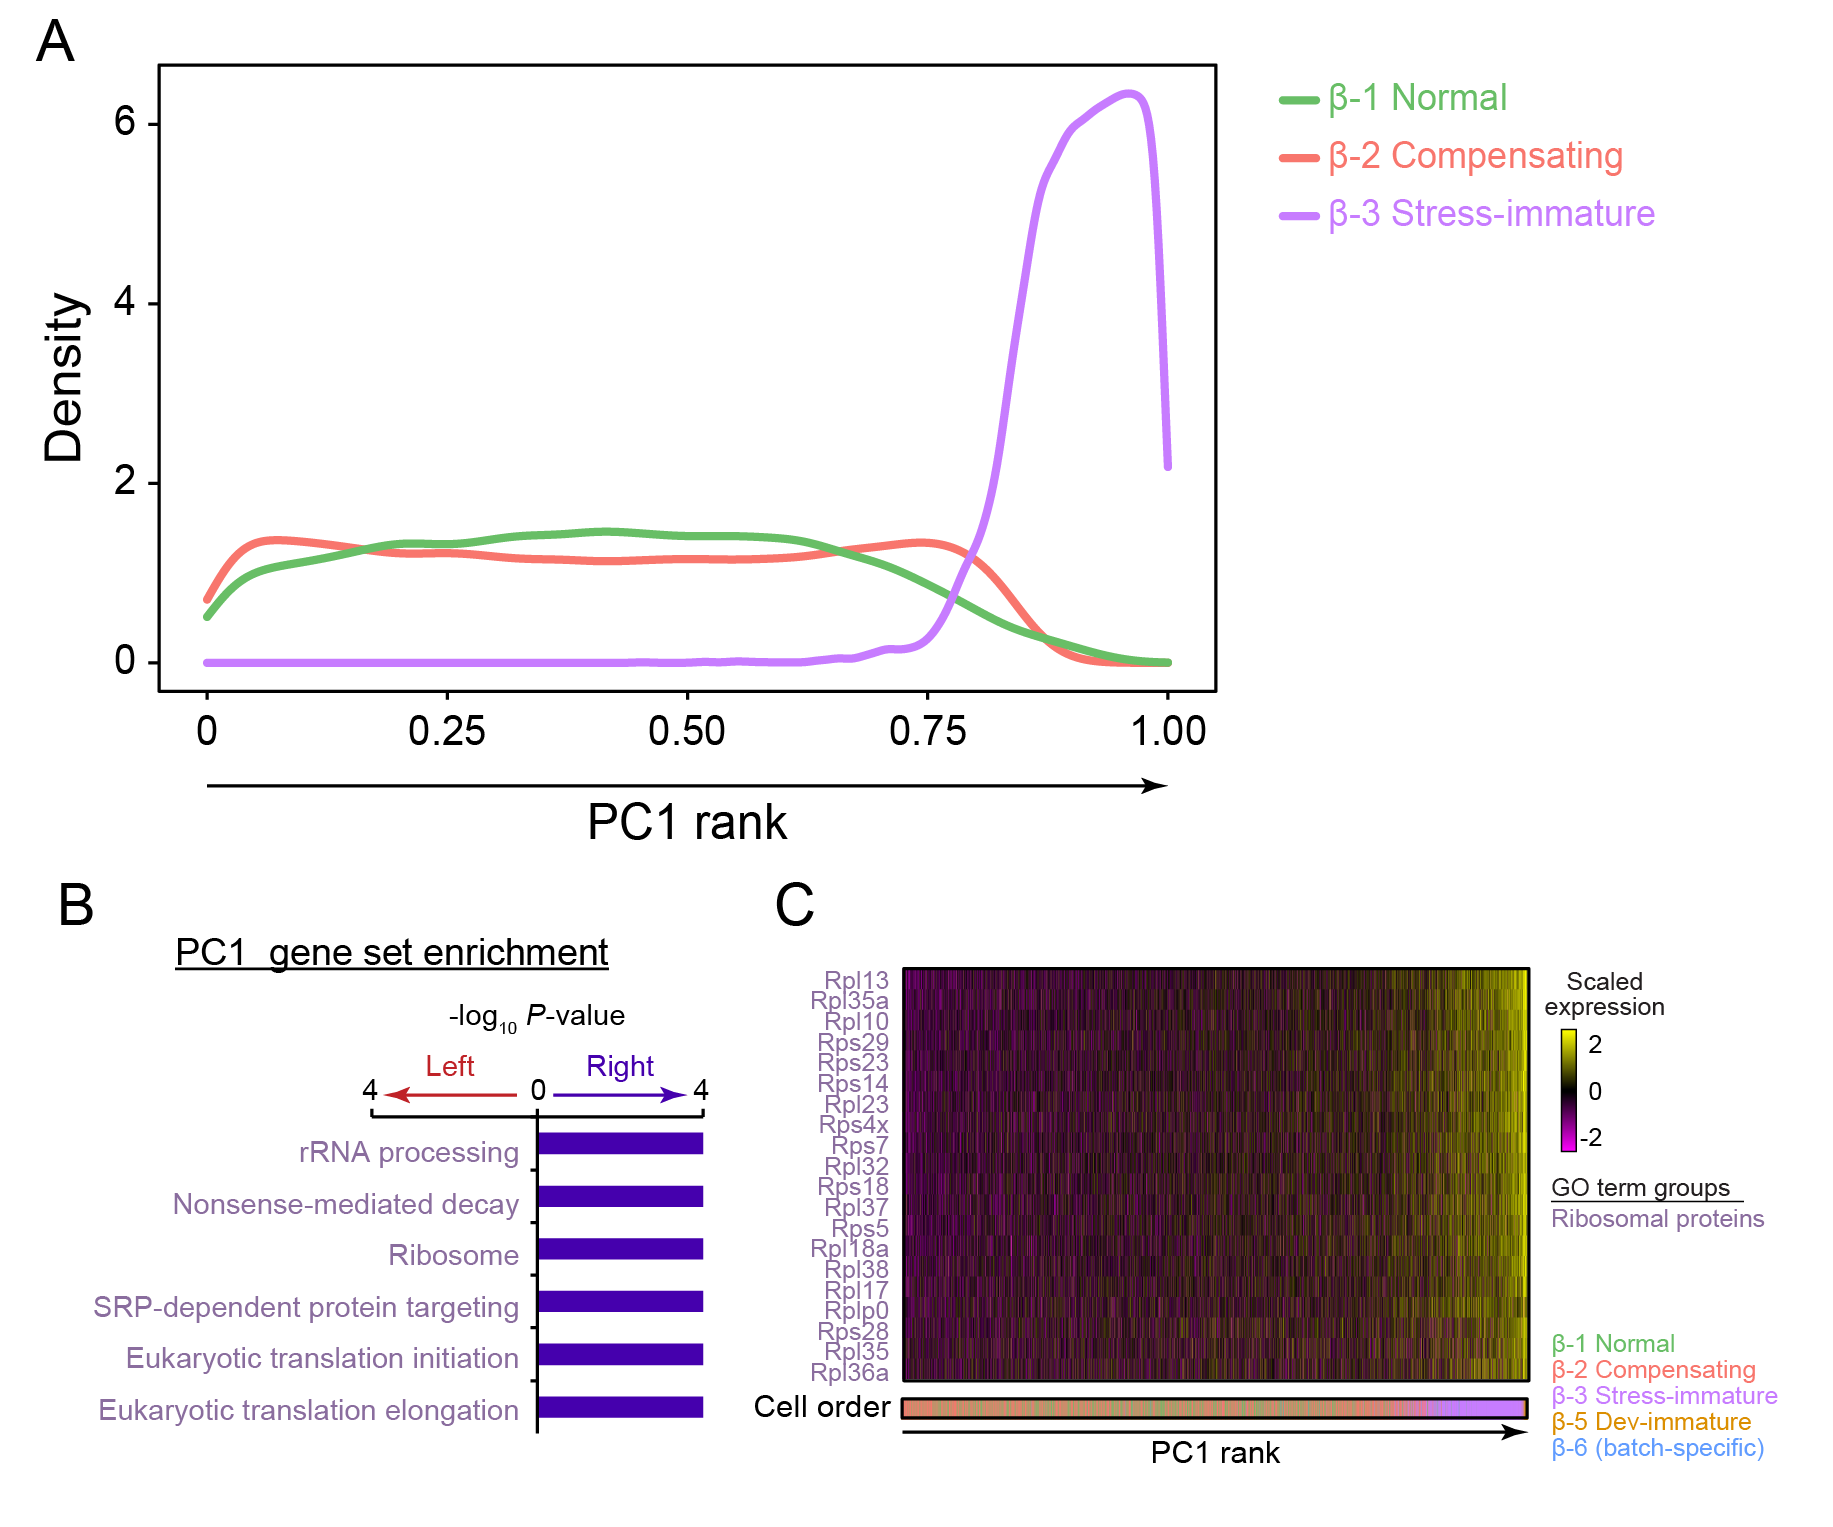
\includegraphics[width=\linewidth]{Chapter5/Fig/F3-6-02}
\caption[Deteriorating glucose homeostasis associates with PC1]{\textbf{Deteriorating glucose homeostasis associates with PC1}\\}
\label{fig:3-6}
\end{figure}


A shifted distribution of cells along PC1 across the experimental interventions depicted that the loss of β-cell maturity occurred in models with systemic hyperglycemia i.e., in \textit{ob/ob} mice and following S961- or \gls{stz}-treatment \textbf{(Fig. \ref{suppl_fig:chp3_pc1} B, \textit{bottom row})}. This was in contrast to the modest interventions which resulted in successful β-cell adaptation, wherein there were minor differences surrounding β-cell immaturity in feeding, WD-induced obesity or the \textit{db/db} mice \textbf{(Fig. \ref{suppl_fig:chp3_pc1} B, \textit{top row})}. Overall, this observation supports that β-cell decompensation associates with loss of maturity. In addition to the upregulation of genes involved in OxPhos and protein processing in the ER in β-3 and β-5 subsets \textbf{(Fig. \ref{fig:3-4} B)}, \gls{pc}1 also corresponded with the upregulation of ribosomal protein genes \textbf{(Fig. \ref{fig:3-6} B,C)}.\\ %\st{This could be explained by a higher demand for protein synthesis in β-3 subset in order to adapt to increased workload demands associated with hyperglycaemic environment and β-5 subset wherein cells could be producing a large number of ribosomes in order to support the synthesis of proteins required for maturation.}\\


%\clearpage

On the other hand, \gls{pc}2 explained 12\% of the variance across β-cell subsets \textbf{(Fig. \ref{fig:3-5})} and corresponded with increased insulin demand per β-cell \textbf{(Fig. \ref{fig:3-7}, Fig. \ref{suppl_fig:chp3_pc2})}. The ‘ranked’ histogram plot of the cells ordered by their PC2 weights distinguished β-1 Normal cells from β-2 or β-3 subsets. Further, the cell distributions across the PC2 rank was shifted for all experimental interventions, including fasting and refeeding. Thus, PC2 seemed to describe the extent of workload with respect to any model that increased insulin demand on a per β-cell basis, which can be impacted through either altered insulin sensitivity or altered β-cell numbers. Compared to PC1, diverse gene-sets were associated with PC2 progression with the apparent repression of mitochondrially-encoded components of the electron transport chain (ETC) and upregulation of genes involved in proteostasis and the glycosylation machinery. We speculate these changes reflect activation of a program intended to preserve ER homeostasis when each cell is attempting to produce and secrete increasing amounts of insulin.\\

\begin{figure}[H]
\centering
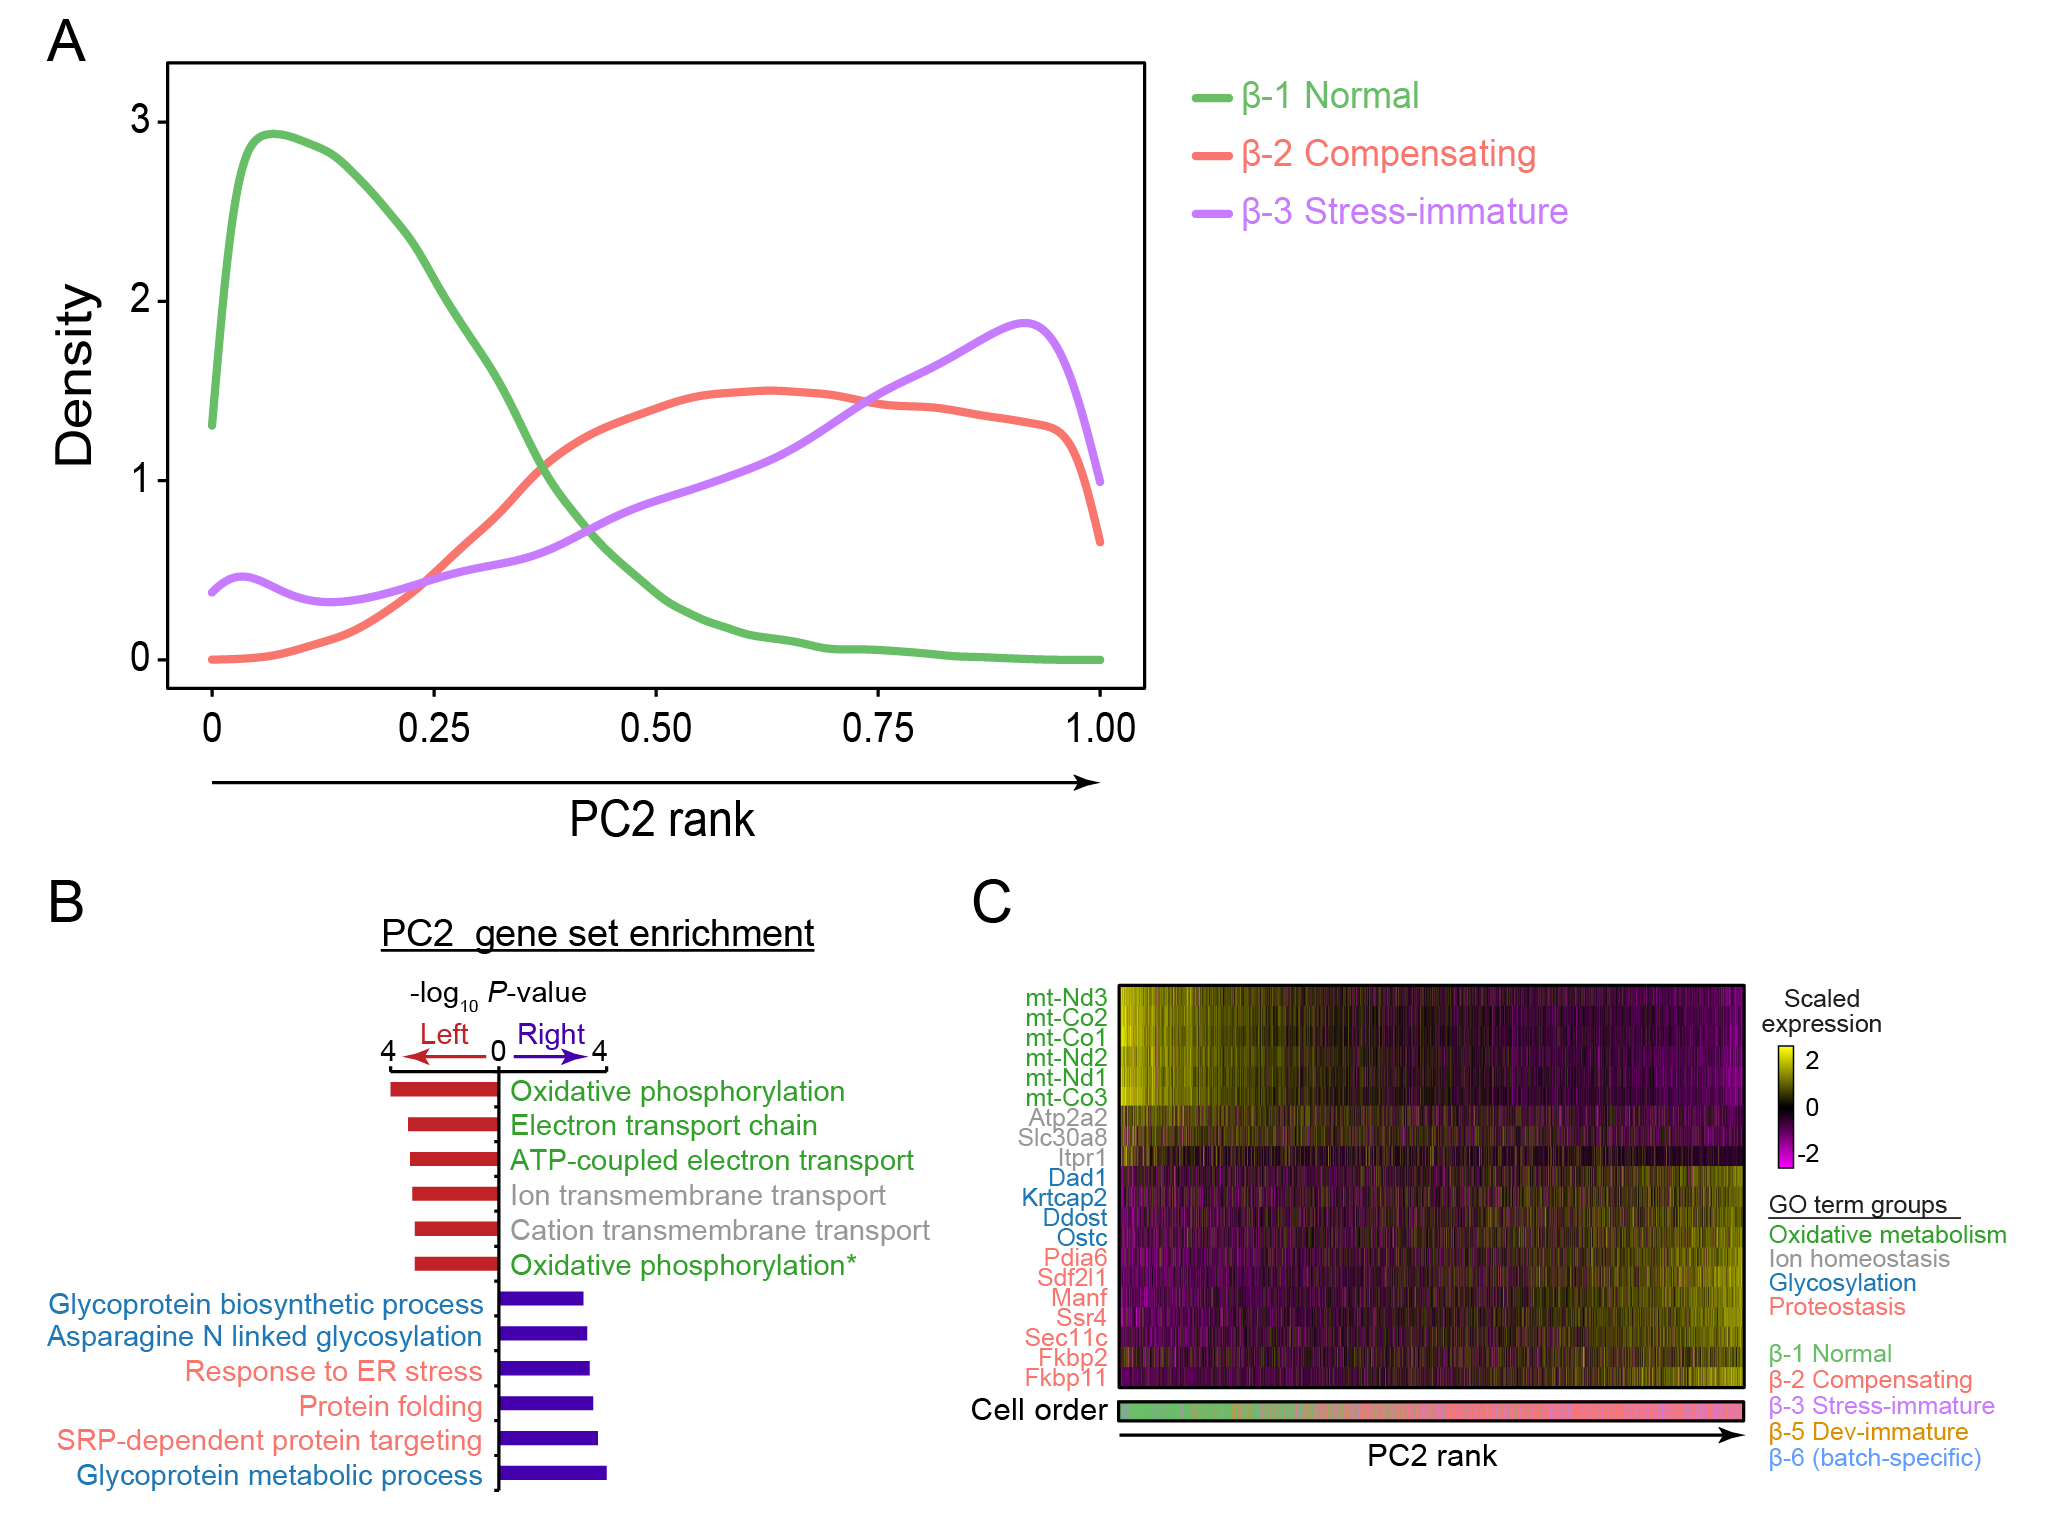
\includegraphics[width=\linewidth]{Chapter5/Fig/F3-6-03}
\caption[Increased β-cell workload associates with PC2]{\textbf{Increased β-cell workload associates with PC2}\\}
\label{fig:3-7}
\end{figure}

\clearpage

% \begin{wrapfigure}{l}{0.7\textwidth}
% 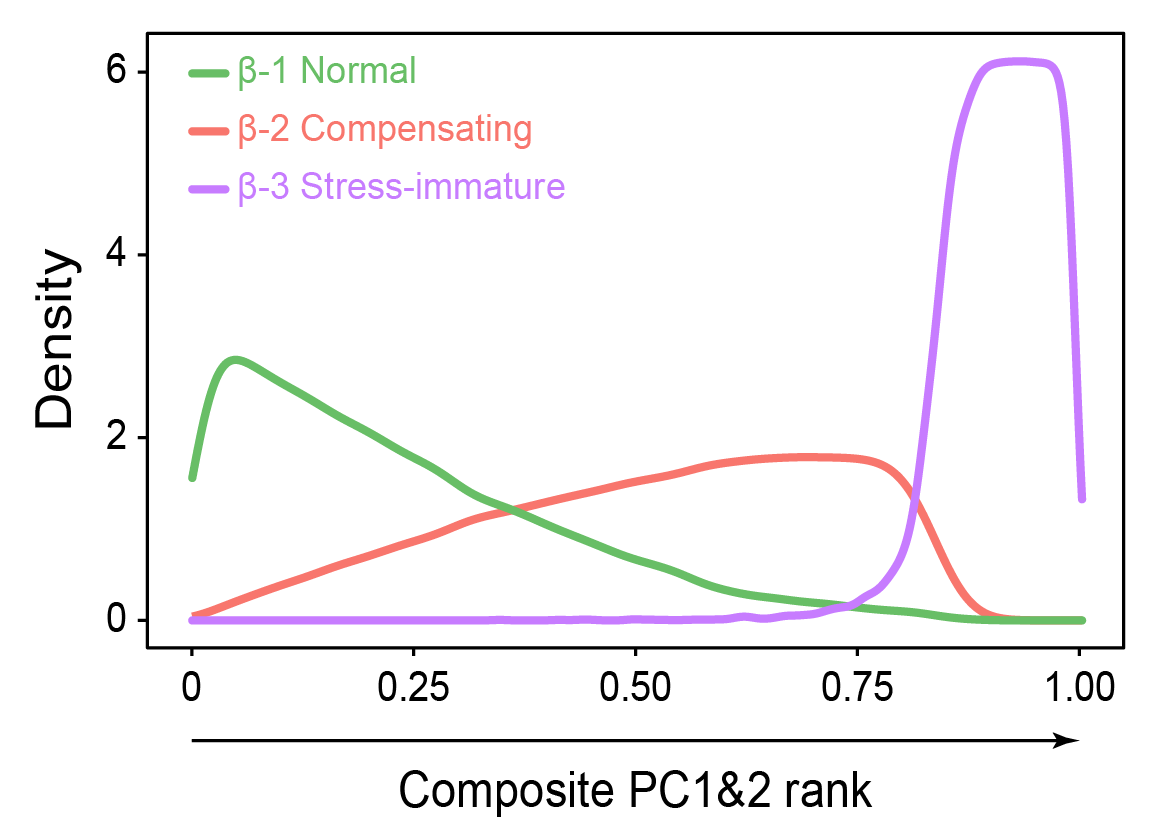
\includegraphics[width=10cm]{Chapter5/Fig/F3-6-04.png}
% \caption[Composite PC1 \& PC2]{}
% \label{fig:3-8}
% \end{wrapfigure}



Combining PC1 and PC2, we hypothesized that the three major subsets could be better represented along a composite axis that encompasses a degree of maturity (PC1) and a degree of workload (PC2). The β-1 Normal subset progressively switches to β-2 Compensating subset along the Maturity-Workload axis, therefore indicating that β-1 and β-2 could rather be continuous phenotypes as opposed to two discrete subsets. β-2 Compensating cells exhibit signatures of increased workload but still retain β-cell identity. β-3 Stress-Immature subset, on the other hand, are exposed to increased insulin demand and also lose their mature identity, thereby distinguishing these cells which are in a decompensated state, resulting in hyperglycemic phenotypes.


\mysidecaption{0.4}{%
\captionof{figure}[Trajectory of β-cell failure along PC1 and PC2]{\textbf{β-cell failure corresponds to increased workload concomitant with loss of maturation}}%
}
{%
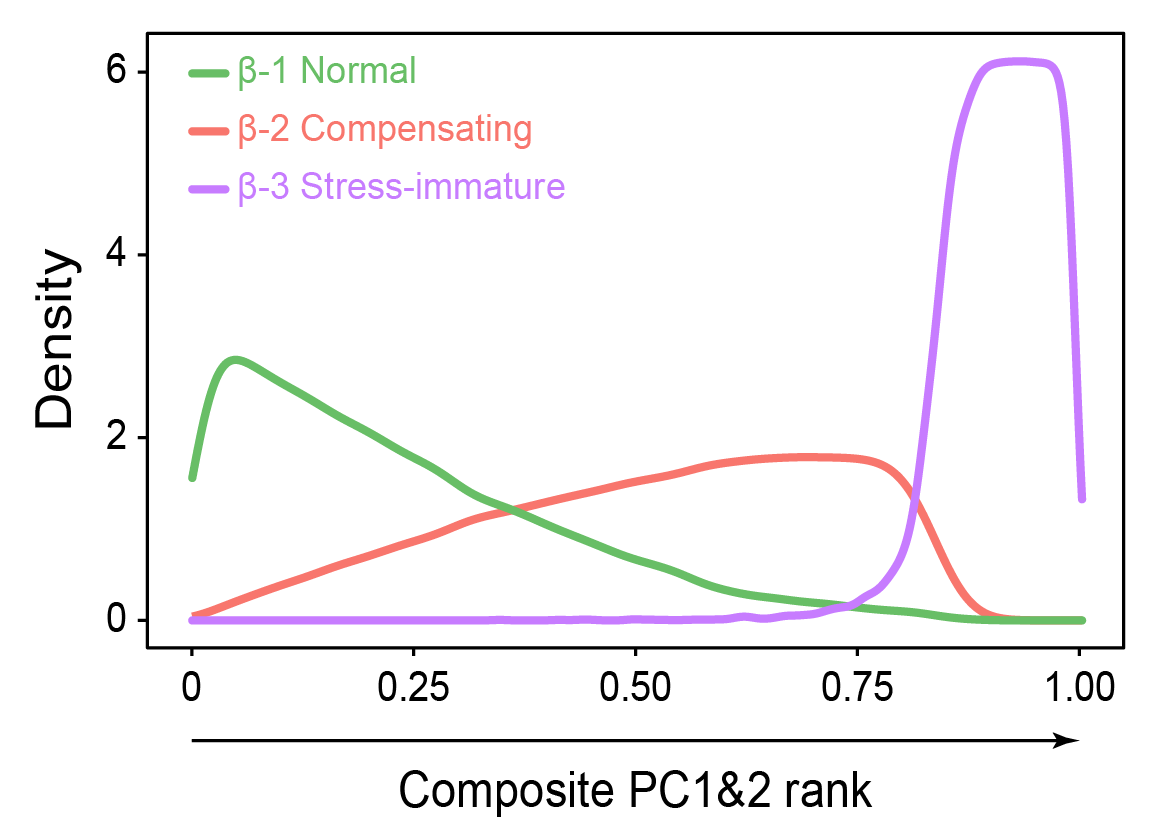
\includegraphics[width=9cm,height=9cm,keepaspectratio]{Chapter5/Fig/F3-6-04.png}%
}[t]%

\hl{\\\\In summary ...}

\clearpage

\section{}
\label{sec:chp3_betaGRN}
Unraveling the complex web of \glspl{grn} is fundamental to decoding the complex regulatory mechanisms that govern cellular response to environmental cues. As already discussed, the development and maturation of β-cells is tightly regulated by the coordinated activity of several key TFs (\textit{Pdx1, Mafa} and \textit{Nkx6-1}), that target several genes, in order to maintain normal β-cell identity and function. However, very little know is about how TFs in β-cells are affected in response to increasing workload, and how they govern state transitions in an interconnected, heterogeneous manifold. Therefore, to understand the molecular mechanisms that underlie these transcriptional differences, we performed \gls{grn} analysis using pySCENIC to infer TF activity and infer \gls{tf}-specific \glspl{grn}. A description of the workflow for \gls{grn} inference using the SCENINC workflow can be found in \hyperref[sec:scrna_analysis_grn]{Section 1.5.6}.\\

% \begin{wrapfigure}{r}{0.8\textwidth}
% \centering
% 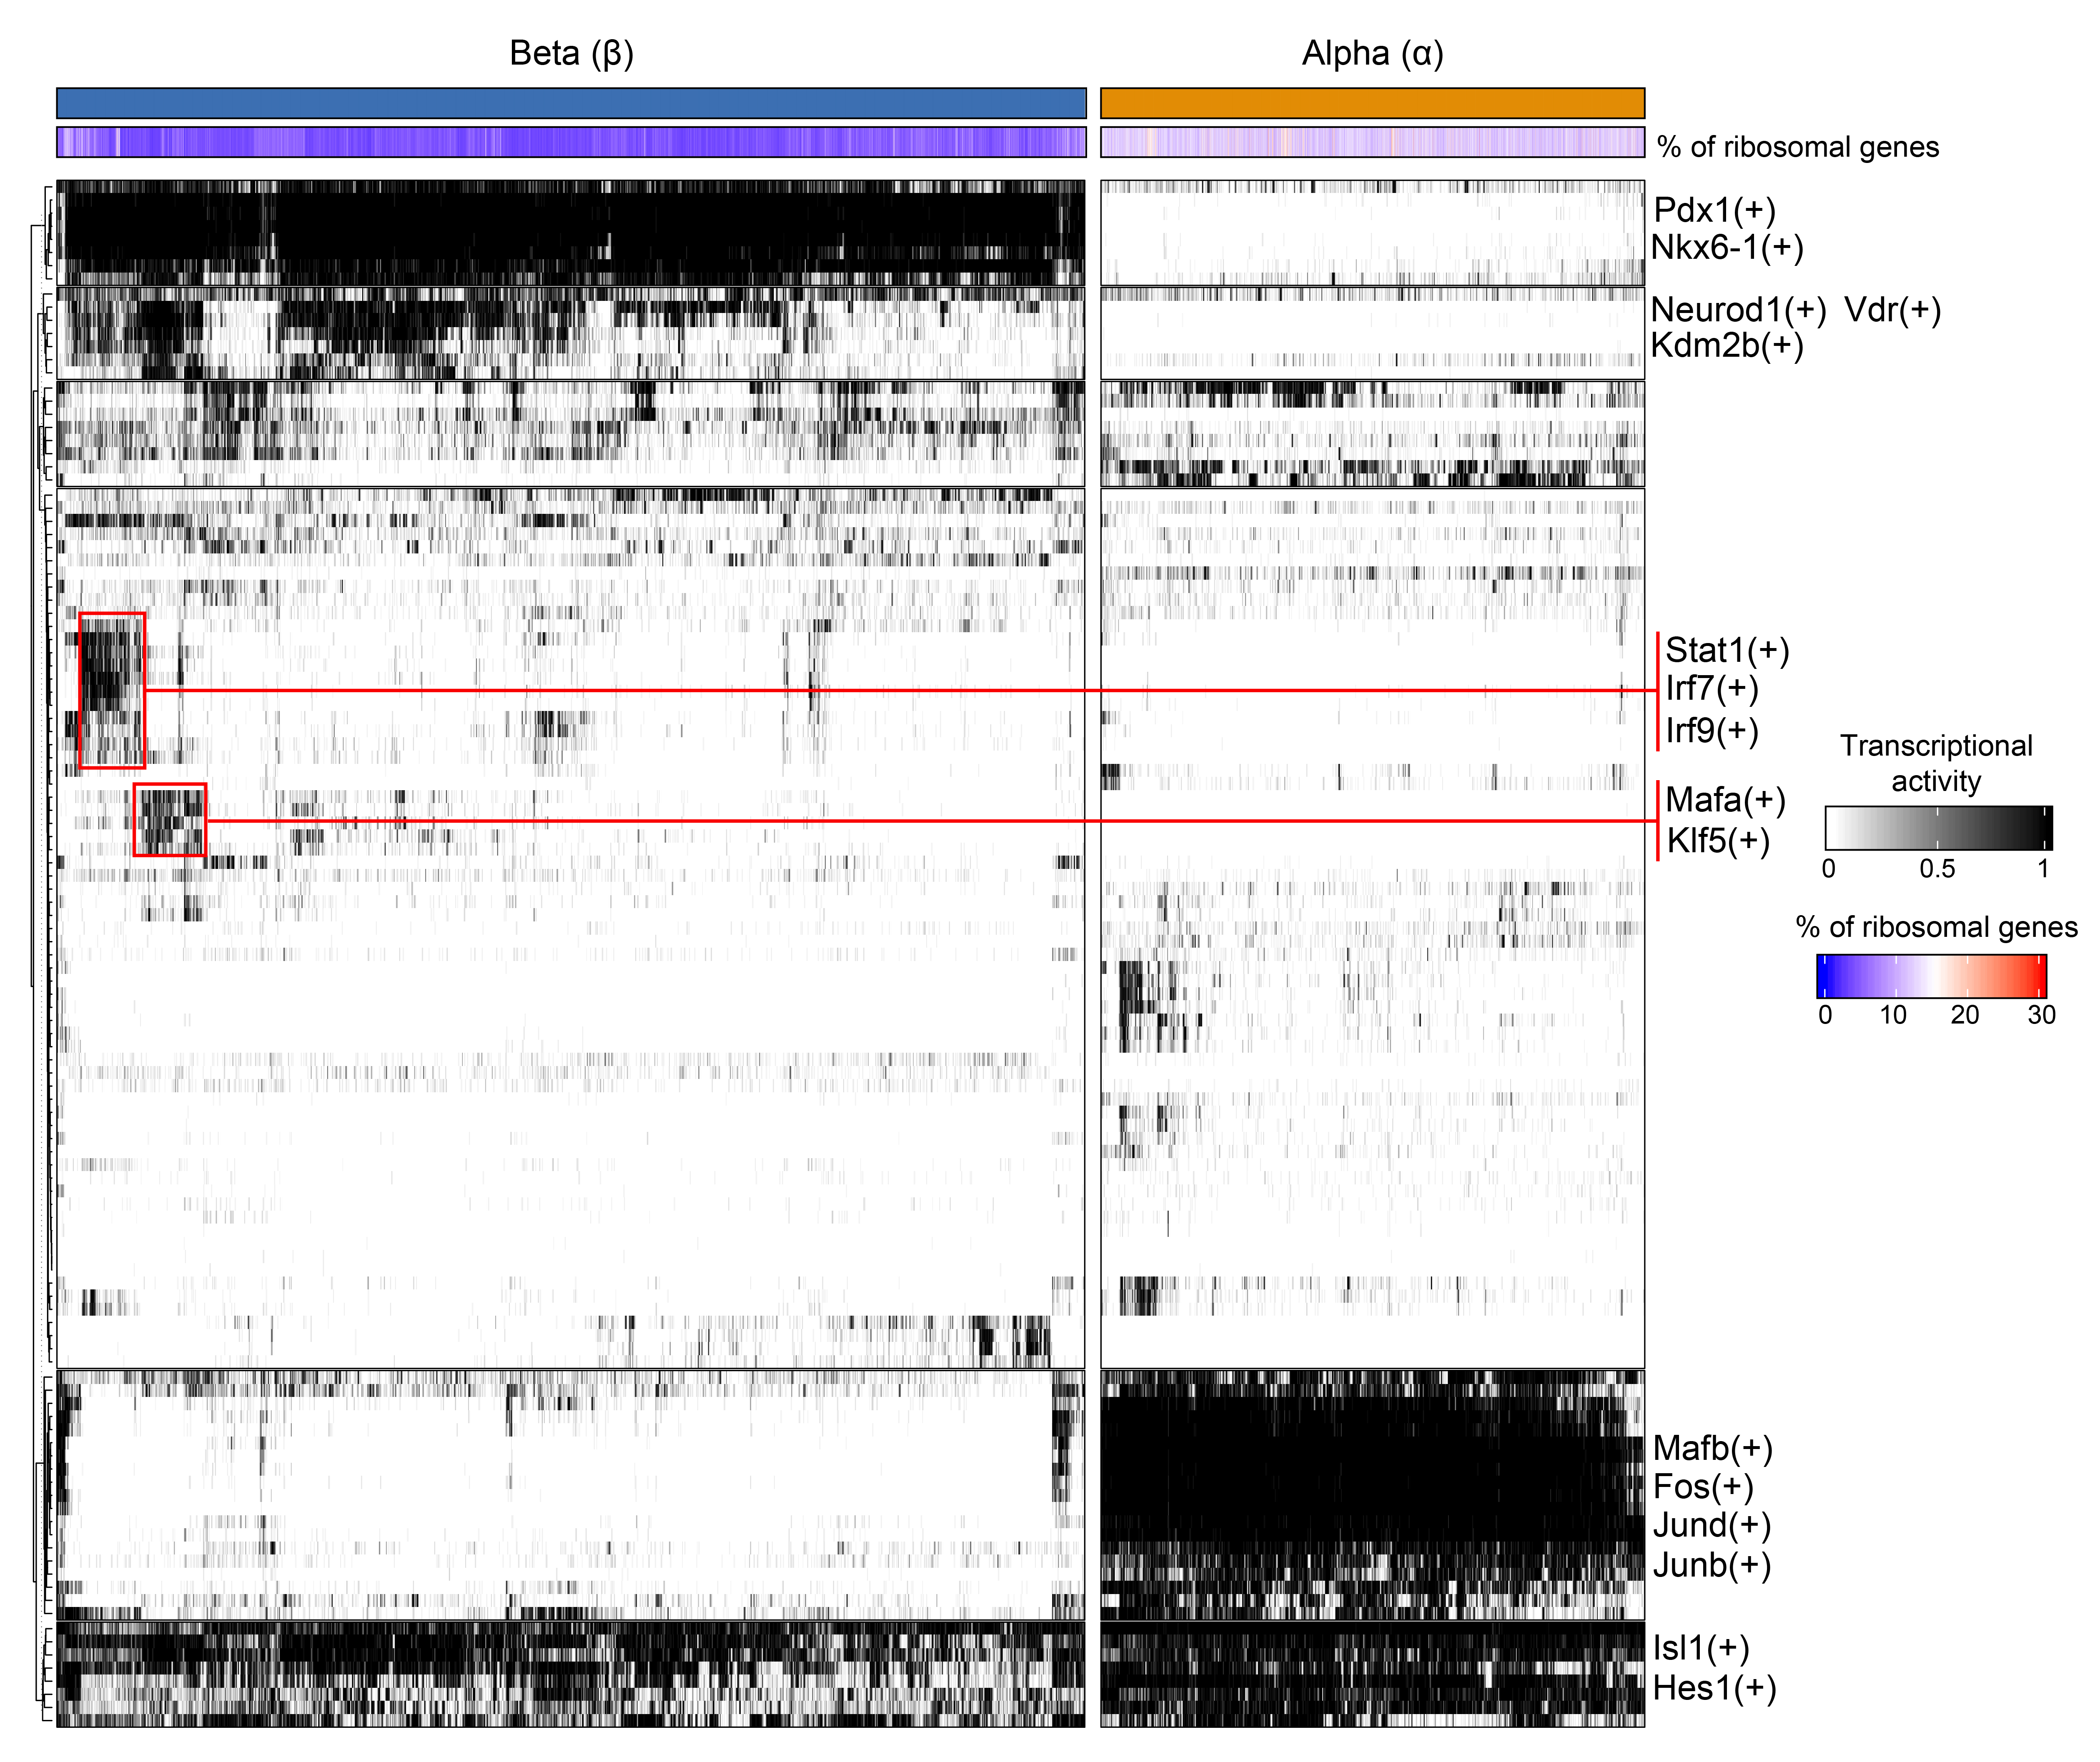
\includegraphics[width=12cm]{Chapter5/Fig/F3-11-01.png}
% \caption[Identification of cell-type specific regulons]{\textbf{Identification of cell-type specific regulons}\\Heatmap depicting the binarized AUC scores, representing the transcriptional activity of regulons across all the cells. Regulons shown in black are considered "ON", while regulons in white are considered "OFF". Top row shows the distribution of cells in the heatmap subdivided by cell-type and percentage of ribosomal genes.}
% \label{fig:3-11}
% \end{wrapfigure}

We applied pySCENIC to the two largest islet cell-types in our data: Alpha and Beta. We subset cells annotated as `Alpha' from \textbf{(Fig. \ref{fig:3-2} A)} and re-integrated with the non-proliferating β-cells. We then applied pySCENIC to this two cell-type re-integrated subset in order to identify α-cell and β-cell specific regulons \textbf{(Fig. \ref{fig:3-11})}. As expected, we identified \textit{Pdx1, Nkx6-1 and Mafa} in β-cells and \textit{Mafb} in α-cells. We found the \textit{Isl1} regulon to be active in both cell-types, which is regarded as a candidate TF regulator in islet cell lineage [\href{https://www.ncbi.nlm.nih.gov/pmc/articles/PMC2551686/}{here}] and controls pancreatic alpha cell fate and β-cell maturation [\href{https://www.ncbi.nlm.nih.gov/pmc/articles/PMC9999528/}{here}]. In addition, \textit{Hes1}, a downstream target of \textit{Notch}, was also active in both the cell-types.\\\\
In β-cells, we identified 124 regulons across the five non-proliferating subsets. \glspl{tf} often work in coordination to regulate gene expression levels. Therefore, to determine the degree of TF activity coordination in mouse β-cells, we computed the connection specificity index (CSI) on the basis of pairwise comparisons of regulon activity patterns across cells, and identified five modules with varying number of regulons \textbf{(Fig. \ref{fig:3-10} A, Supplementary Table \ref{tab3-2})}. We also visualized the transcriptional \gls{grn} underlying the non-proliferating β-cells by using the top 1\% of the reported \gls{tf}-target associations based on the importance metric (IM) from the pySCENIC analysis \textbf{(Fig. \ref{fig:3-10} B)}.\\


\begin{figure}[t]
\centering
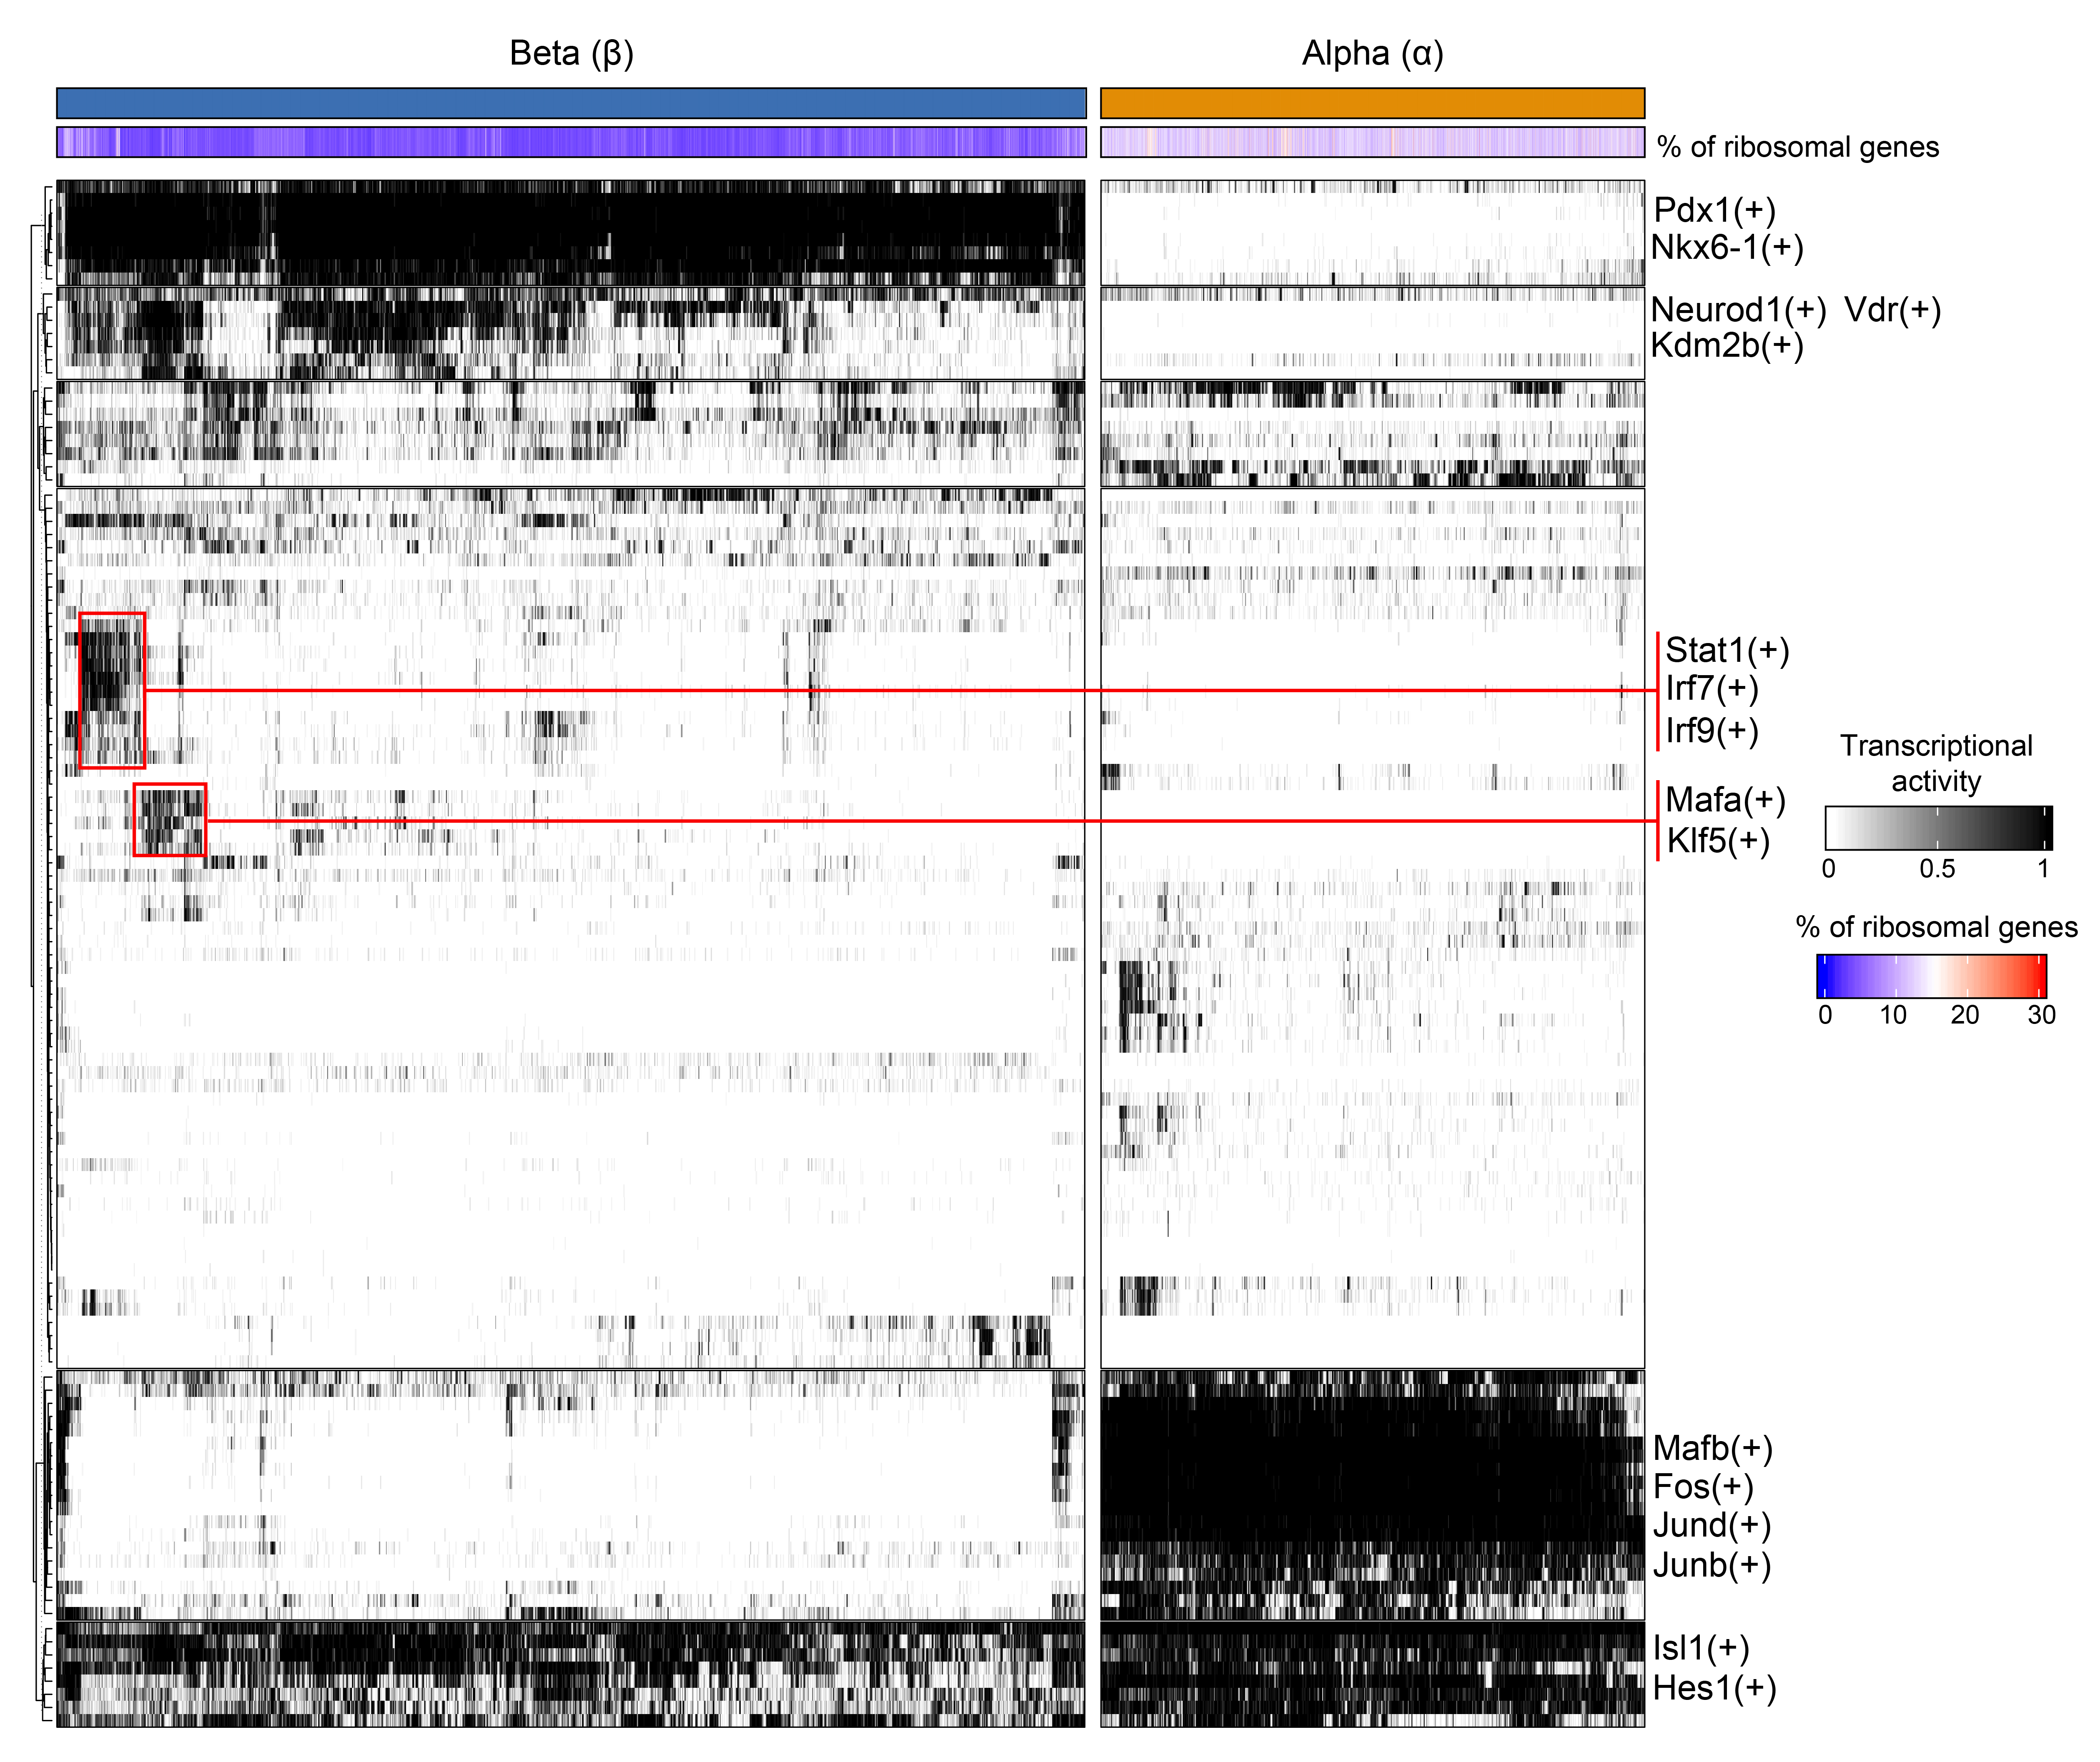
\includegraphics[width=\linewidth]{Chapter5/Fig/F3-11-01.png}
\caption[Identification of cell-type specific regulons]{\textbf{Identification of cell-type specific regulons}\\Heatmap depicting the binarized AUC scores, representing the transcriptional activity of regulons across all the cells. Regulons shown in black are considered "ON", while regulons in white are considered "OFF". Top row shows the distribution of cells in the heatmap subdivided by cell-type and percentage of ribosomal genes.}
\label{fig:3-11}
\end{figure}

The largest module, \textit{Module 1}, contained TFs associated with β-cell function (\textit{Mafa, Nkx6-1}) and development (\textit{Neurod1, Pdx1}) \textbf{(Fig. \ref{fig:3-10})}. The mean regulon activity of \textit{Mafa} and \textit{Pdx1} was comparable across all subsets \textbf{(Fig. \ref{fig:3-12})}. The activity of \textit{Tcf7l2}, a master regulator of insulin production and processing, and its downstream target \textit{Isl1} were also similar across all subsets. Interestingly, the mean activity of \textit{Neurod1} regulon was (quantitatively) higher for β-1 Normal subset and was downregulated in β-2 and β-3 subsets. Another interesting TF-regulon with similar activity and expression pattern is \textit{Kdm2b}. \hl{<Stuff about \textit{Kdm2b}>}. Module 1 also included \textit{Atf5}, which has been shown to be an important regulator of ER stress and apoptosis in mouse β-cells \textbf{\cite{ma_atf5_2023}}, and \textit{Hmgb1}, a chromatin protein that can induce autophagy by activating various pathways and has been shown to play an important role in insulin resistance and diabetes \textbf{\cite{yang_relationship_2023}} \textbf{(Fig. \ref{fig:3-12})}. \hl{<Stuff about \textit{Vdr}>}\\

\textit{Module 2} was characterized by the presence of \textit{Fos} and \textit{Jun} regulons, which are components of the activator protein-1 (AP-1) TF complex, and are involved in stress response and have been implicated in the regulation of β-cell function, particularly under conditions of metabolic stress or diabetes. \textit{Jund}, a member of the \textit{Jun} family, in particular,  has been found to be upregulated  in response to high concentrations of glucose and free fatty acids, and its depletion can block the increase in oxidative stress and apoptosis in β-cells during glucolipotoxicity \textbf{\cite{good_jund_2019}}. Strikingly, this module also contained the TF \textit{Arx}, which specifies the formation of pancreatic islet α-cell during development. The \textit{Arx} regulon was active in both, the β-3 Stress-immature and the β-5 Dev.-immature subsets. The higher activity of \textit{Arx} in β-3 compared to β-1 or β-2 subsets likely suggests the activation of a dedifferentiation like-program in response to increased workload in hyperglycemic and insulin-resistant models. The forced over-expression of \textit{Arx} within pancreata showed massive reductions in beta and delta cell numbers and increased alpha and PP cell numbers \textbf{\cite{van_der_meulen_role_2015}}. This (trans/de)-differentiation could be mitigated by the activity of \textit{Klf6} regulon, a downstream effector of \textit{Sox9} \textbf{\cite{puri_sox9_2024}} and an immediate early response gene \textbf{\cite{xin_single-cell_2016}}, in β-2 subset, as \textit{Klf6} has been shown to protect β-cells against insulin-resistance induced dedifferentiation. \textit{Klf6} knockout mice displayed stronger β-cell dysfunctions against insulin resistance (WD-feeding) with severe hyperglycemia (S961 treatment) \textbf{\cite{dumayne_klf6_2020}}. \hl{<Stuff about \textit{Taf7,Rorc}>}\\

\begin{figure}[t]
\centering
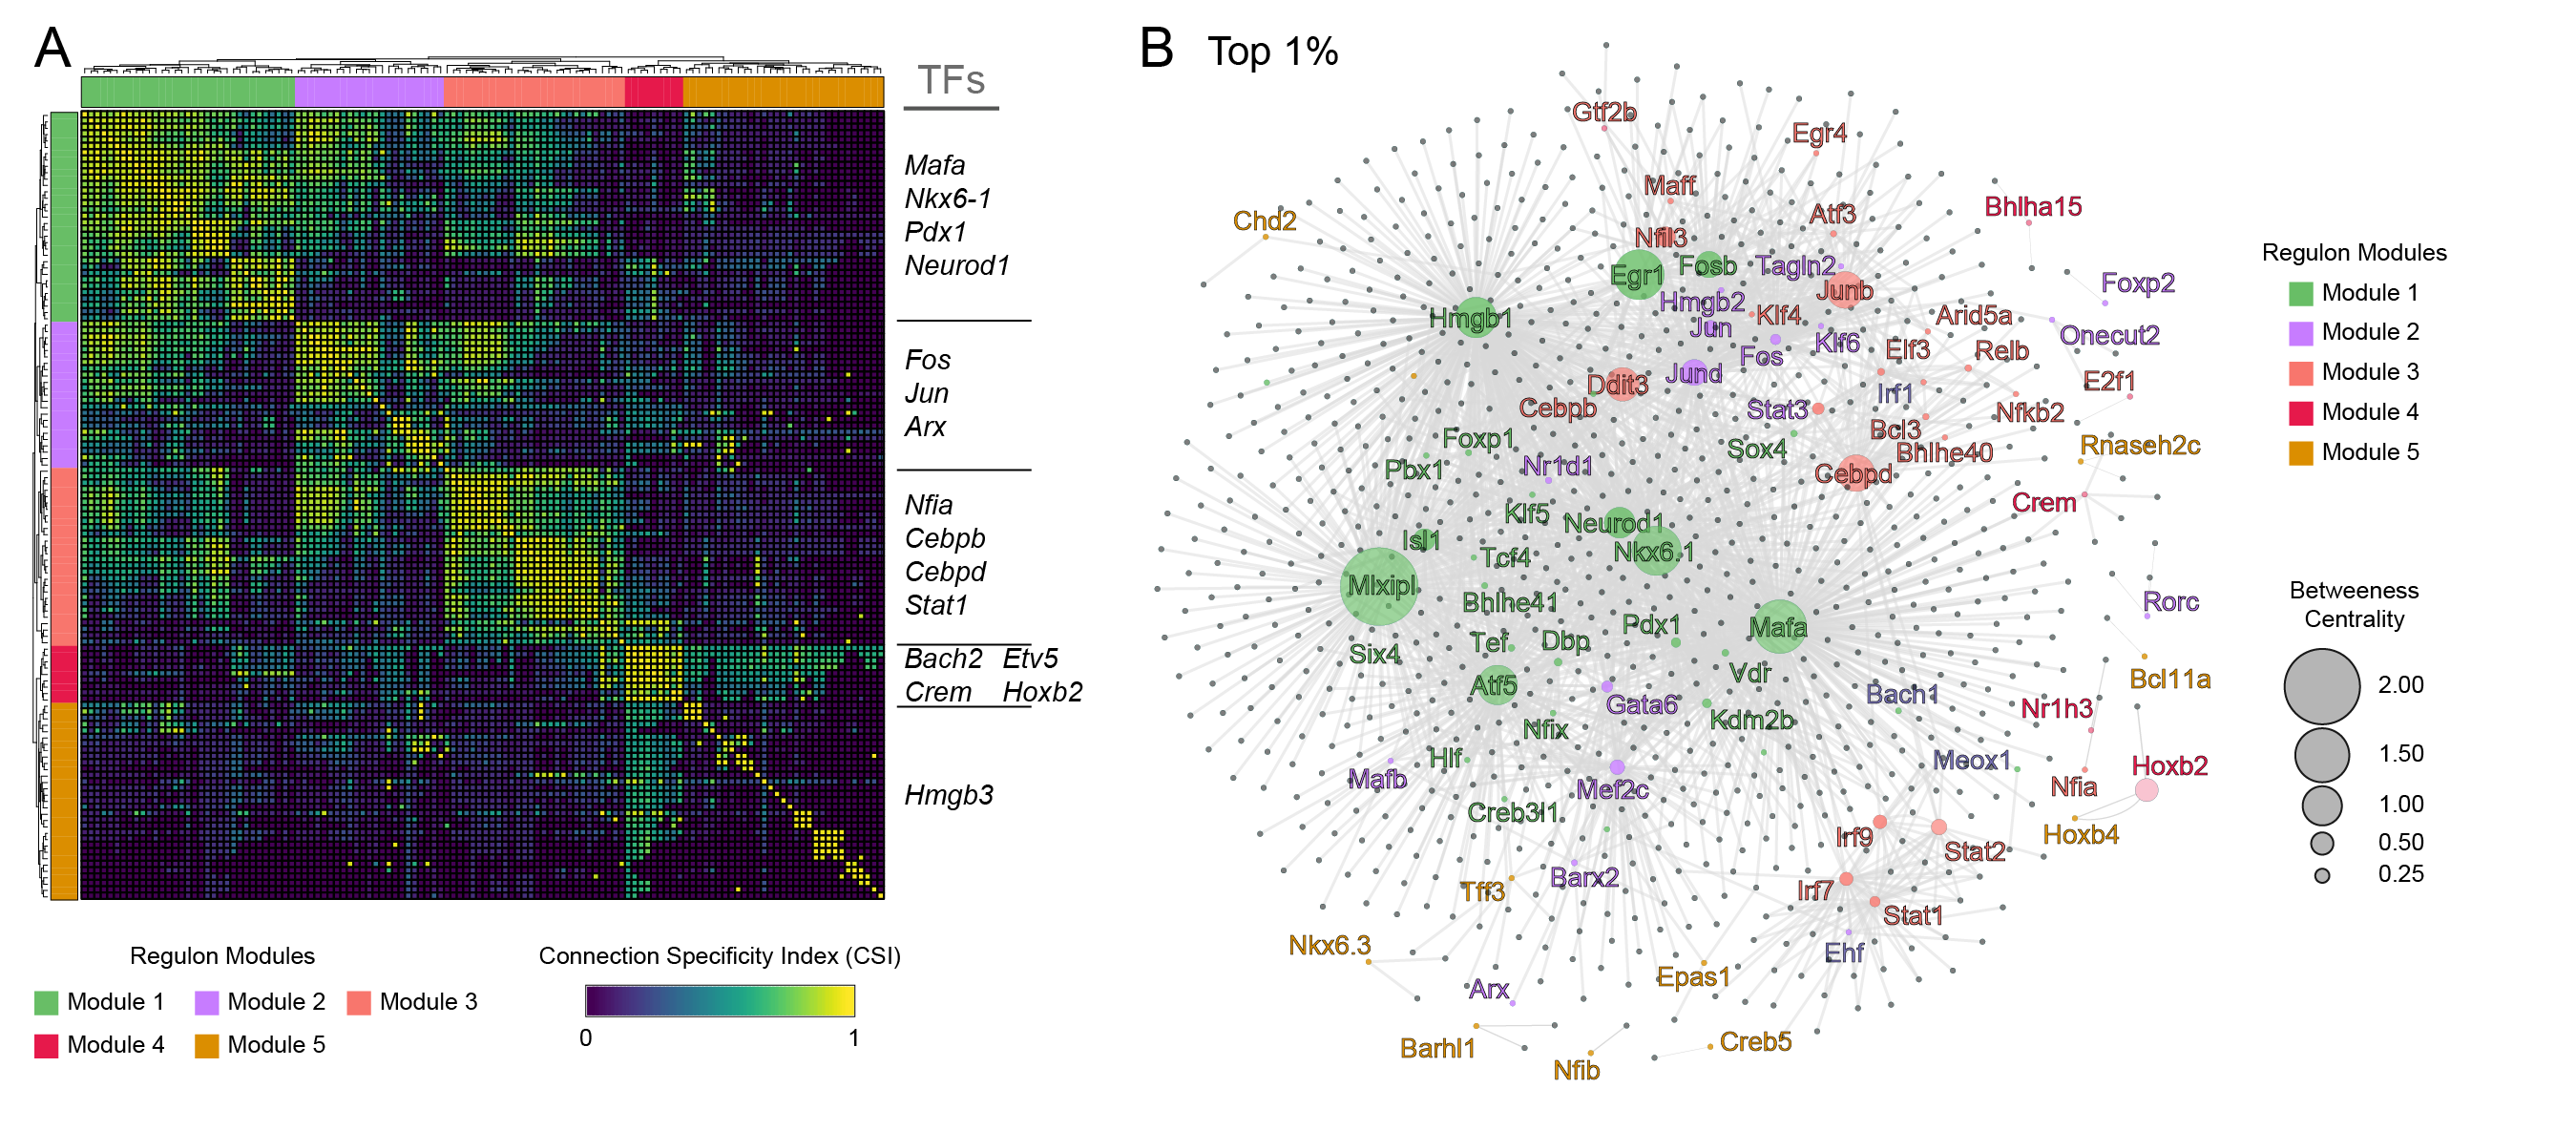
\includegraphics[width=\linewidth]{Chapter5/Fig/F3-10-02.png}
\caption[Identification of β-cell specific GRN and regulon modules]{\textbf{Identification of β-cell specific GRN and regulon modules}\\}
\label{fig:3-10}
\end{figure}

\textit{Module-3} contained the TFs \textit{Cebpb} and \textit{Cebpd}, which have anti-apoptotic and anti-inflammatory roles in pancreatic β-cells \textbf{\cite{https://www.ncbi.nlm.nih.gov/pmc/articles/PMC3275575/}}. This module was also comprised of members of the IFN regulatory factor (\textit{Irf1, Irf7, Irf8} and \textit{Irf9}) and the signal transducer and activator of transcription (\textit{Stat1,Stat2} and \textit{Stat3}) families, which have essential roles in regulating Type-1 IFN induction and downstream actions, respectively \textbf{\cite{https://www.ncbi.nlm.nih.gov/pmc/articles/PMC6331453/}}. In particular, \textit{Stat1} is a master regulator of β-cell apoptosis and islet inflammation \textbf{\cite{https://www.ncbi.nlm.nih.gov/pmc/articles/PMC3020778/}}. Unsurprisingly, the β-1 Normal subset showed higher activity for \textit{Nfia}, which is known to regulate endocrine fate induciton \textbf{\cite{https://www.cell.com/cell-reports/pdf/S2211-1247(18)31869-2.pdf}} and regulates pancreatic physiology through granule recruitment and docking \textbf{\cite{https://www.biorxiv.org/content/10.1101/2019.12.24.885020v1.full}}. \hl{\textit{Module 4} contained regulons such as \textit{Bach2, Bhlha15, Crem, E2f1, Etv5, Gtf2b, Hoxb2, Mybl1, Nr1h3} which seemed to be uniformly active across all β-subsets, whereas most of the regulons in \textit{Module 5} had no activity in any of the β-subsets. Of note, \textit{Hmgb3} regulon had higher activity in the β-5 Dev.-Immature subset compared to the rest and the \textit{Pou6f2} regulon had a similar profile in β-3 Stress-Immature and β-5 Dev.-Immature subsets.}\\


\begin{figure}[t]
\centering
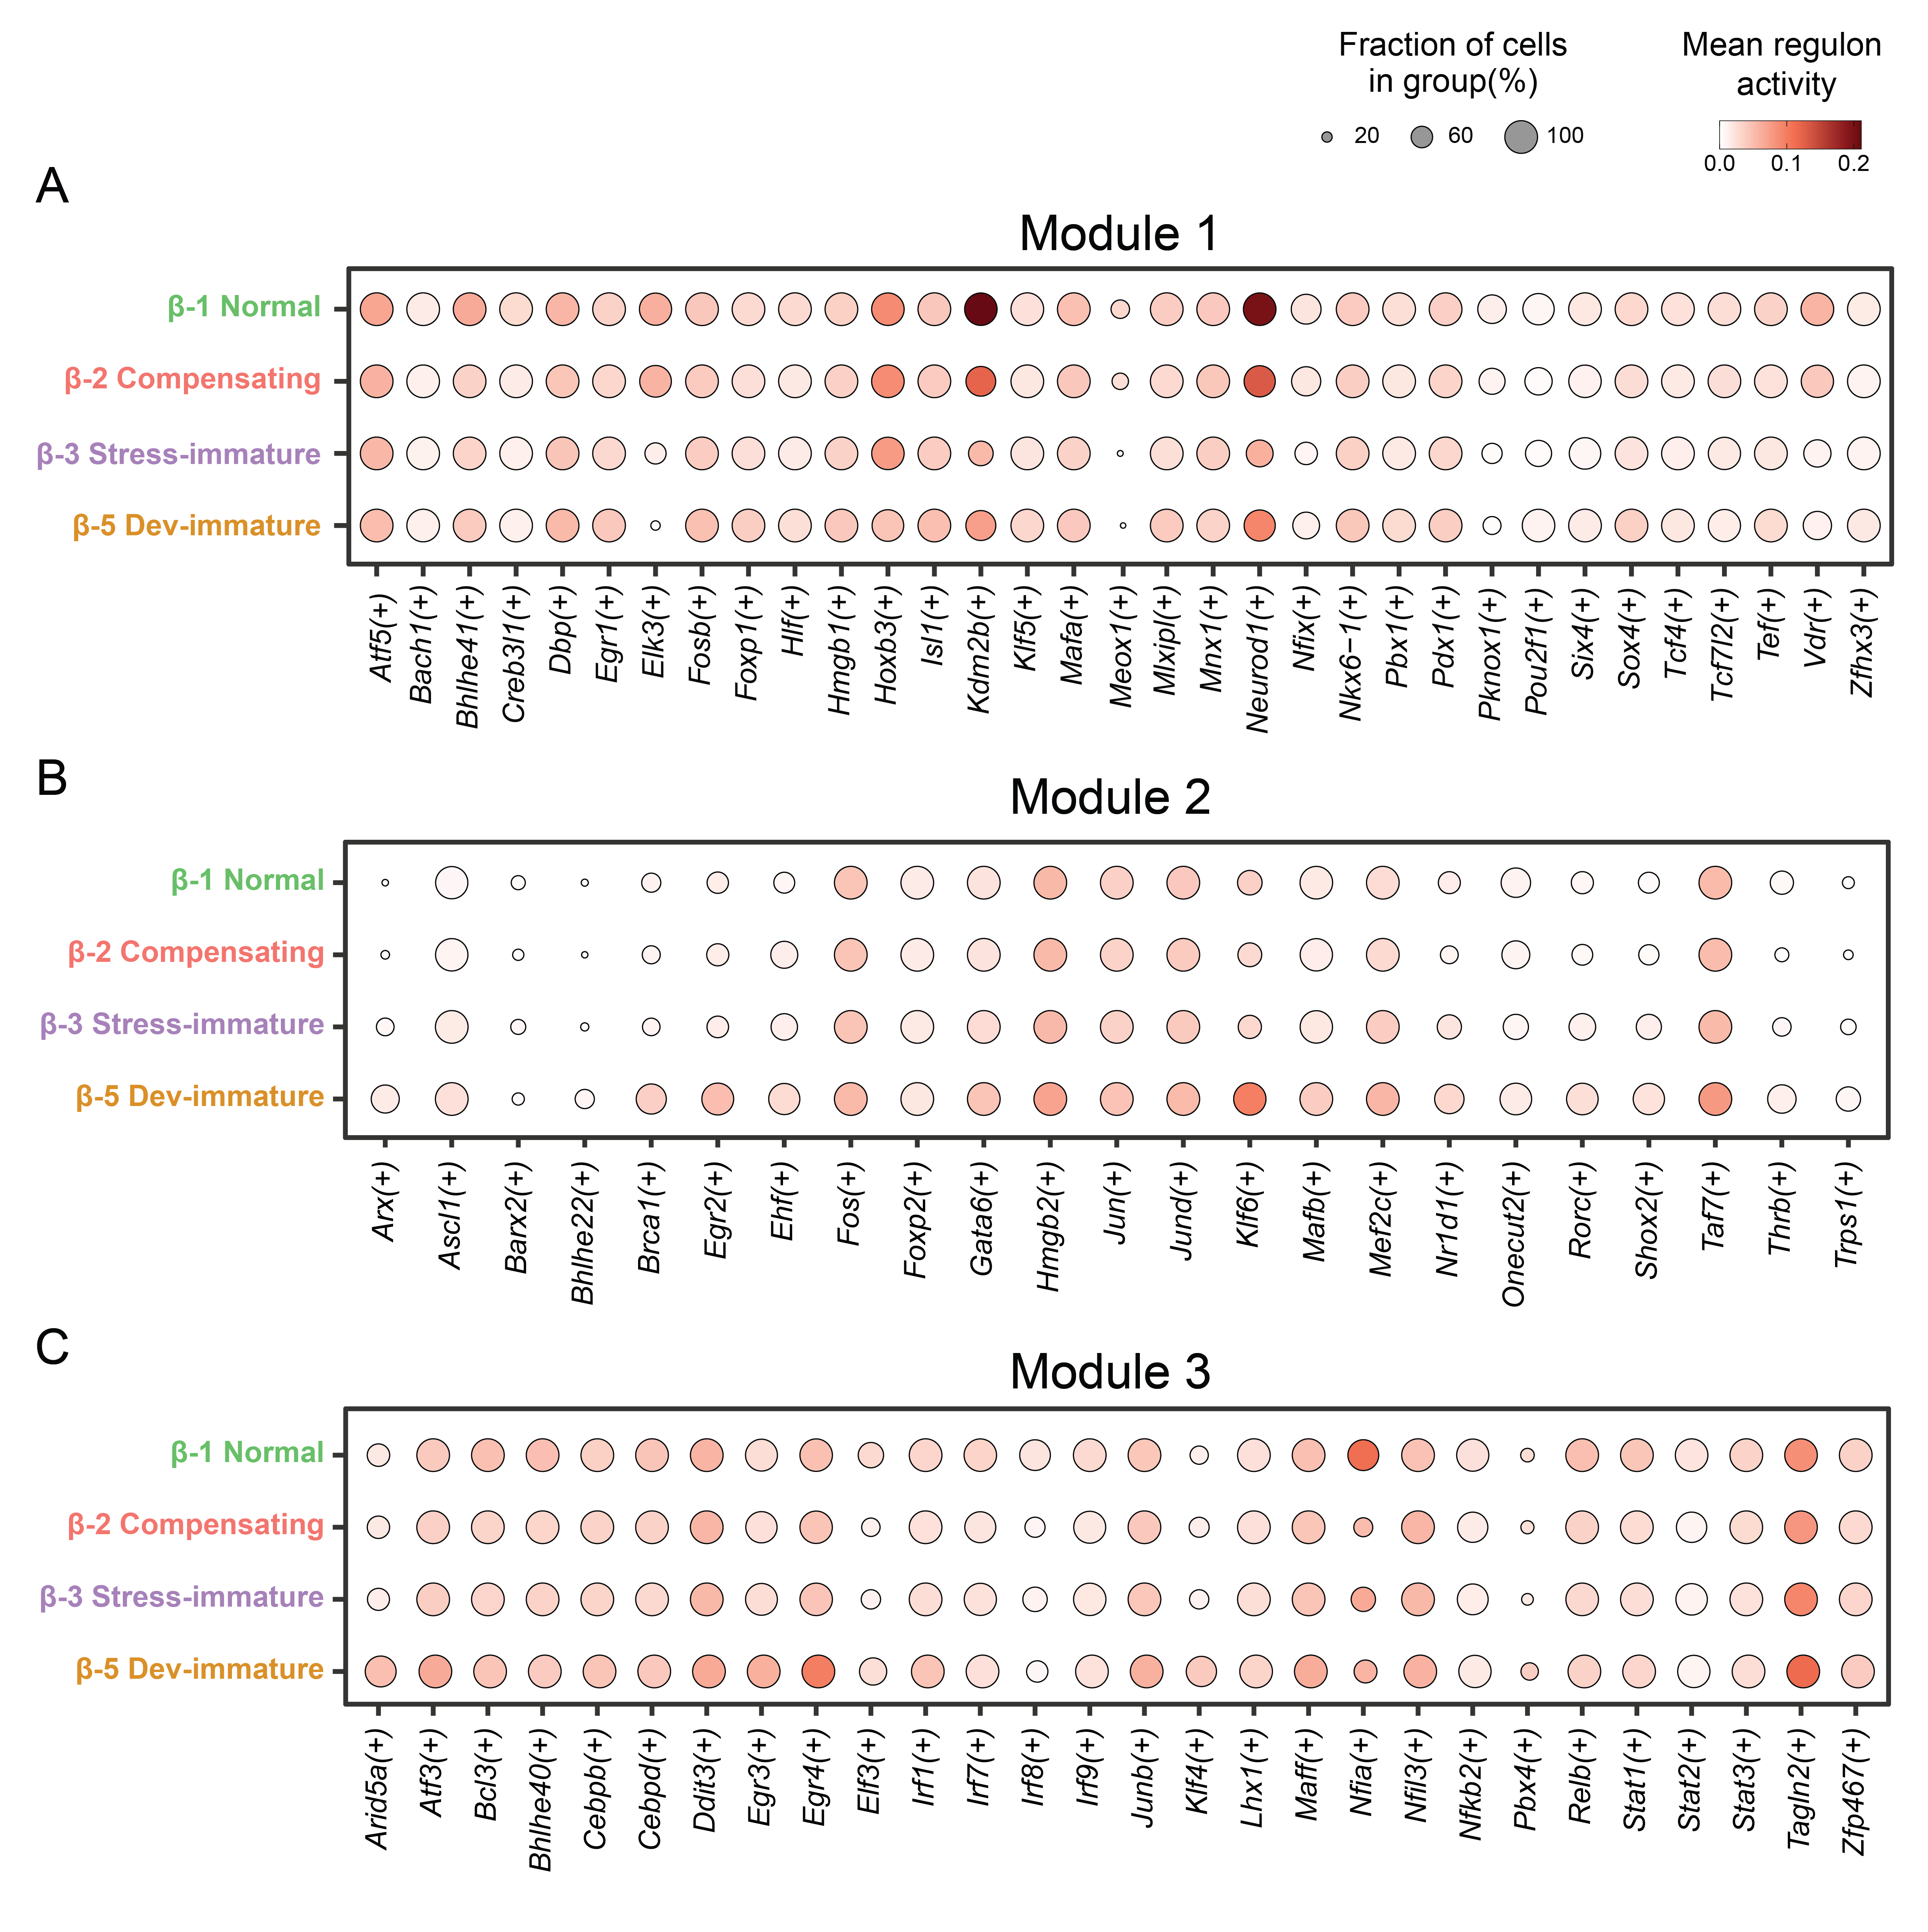
\includegraphics[width=12cm]{Chapter5/Fig/F3-12-03.png}
\caption[Mean regulon activity of all regulons in Module-1 of β-cell GRN]{\textbf{Mean regulon activity of all regulons in Module-1 of β-cell GRN}\\}
\label{fig:3-12-1}
\end{figure}

%\clearpage





% \begin{figure}[H]
% \centering
% \includegraphics[width=\linewidth]{Chapter5/Fig/F3-12-02.png}
% \caption[Mean regulon activity of all regulons in Module-2 of β-cell GRN]{\textbf{Mean regulon activity of all regulons in Module-2 of β-cell GRN}\\}
% \label{fig:3-12-2}
% \end{figure}


To gain a better understanding about the expression dynamics of \glspl{tf} associated with regulons identified in this analysis, we examined the expression of several candidate \gls{tf} across the Maturity (PC1)-Workload (PC2) axis from \textbf{Section \ref{sec:chp3_betaPCA}}. Consistent with previous analysis, \glspl{tf} associated with β-cell function (\textit{Mafa, Vdr}), \textit{Kdm2b, Atf5} were downregulated with loss of β-cell maturity. Conversely, the expression of \glspl{tf} such as \textit{Egr1, Hmgb1, Mafb, Mlxipl} and components of the AP-1 complex were correlated with the stress- and  developmentally- immature β-cell subsets. Interestingly, while the expression of key \glspl{tf} like \textit{Neurod1} and \textit{Nkx6-1} in the β-5 Dev-immature subset is expected, they were also upregulated with the loss of maturity in response to insulin resistance and hyperglycemia. \hl{Along the workload axis, ...}\\\\
\hl{In summary ....}

\clearpage

\section{}
\label{sec:chp3_T2Dgenes}

In the MIA, the authors assessed which mouse models within their integrated data captured the transcriptional signatures akin to human T1D or T2D, by performing DGE analysis on β-cells from several human T1DM or T2DM datasets. Doing so, they identified that the NOD model significantly mirrored the immune gene sets typical of human T1D, while the \textit{db/db} and mSTZ models predominantly exhibited gene expression changes linked to metabolic stress and hormone metabolism, akin to human T2D. Similarly, to further assess the extent of similarity in transcriptional profiles of human T2D and the mouse models included in this meta-analysis, we utilized five of the enriched gene sets from MIA. These included gene sets related to pancreas development, hormone metabolism, ribosome biogenesis, protein or peptide breakdown by proteasome and transport vescile of the constitutive secretory pathways. For each of these gene sets, we first identified the orthologous genes in our mouse dataset and then performed gene-set scoring on a single-cell level.\\

\subsubsection{Endocrine Pancreas Development}
The gene set `Endocrine pancreas development' was downregulated in all datasets compared to their respective controls. This was also observed in the case of the \textit{db/db} animals with established hyperglycemia in the MIA , as well as the mSTZ model (which has been included in this study). However, since this gene set  was enriched among human T2D-upregulated genes, the unexpected direction of the gene set change in the mouse T2D models could be attributed to the diversity of the gene set with genes involved in β-cell maturation as well as β-cell immaturity affecting the scoring. We therefore examined specific genes from this set. The expression of several characteristic β-cell identity and function genes in this set were mildly downregulated in all stress models except the feeding intervention and S961 treatment. Genes such as \textit{Gipr, Neurod1, Nkx2-2, Nkx6-1} were mildly upregulated in the fed mice whereas S961 treatment induced the upregulation of \textit{Foxa2, Insm1, Nkx2-2}  and \textit{Pdpk1}. \hl{Add reasoning}

\begin{figure}[t]
\centering
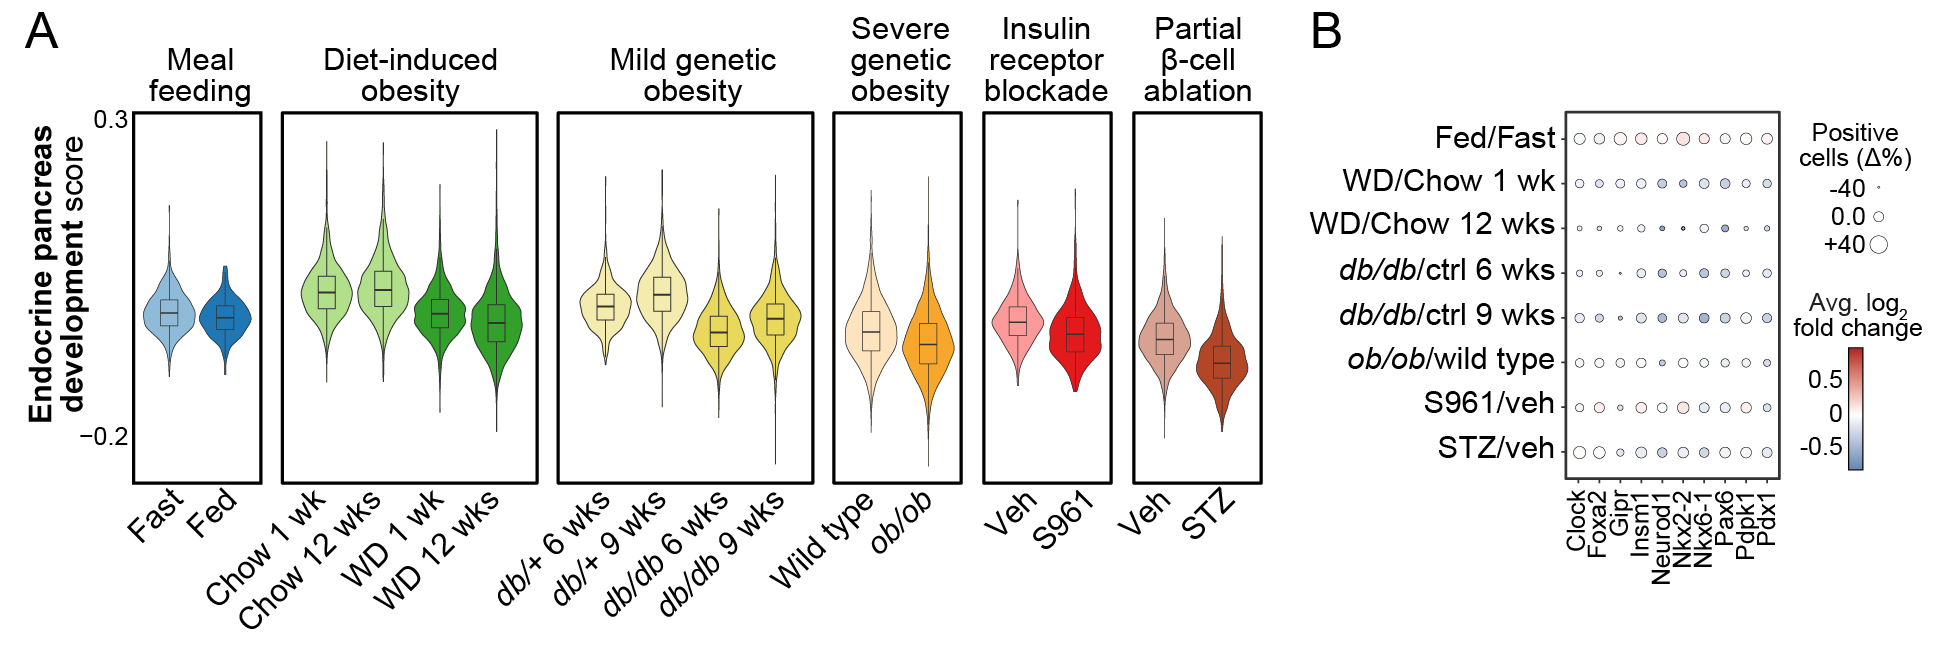
\includegraphics[width=\linewidth]{Chapter5/Fig/F3-13-01.png}
\caption[Gene-set scoring of `\textit{Endocrine pancreas development}']{\textbf{Activity of genes associated with Endocrine pancreas development.} \textbf{(A)} Violin plots depicting the gene-set score for `Endocrine pancreas development' associated genes shown for β-cell workload models and corresponding healthy controls from individual studies. On the overlay boxplots, the middle horizontal line represents the median, the box represents the inter-quartile range and the whiskers represent the minimum and maximum values. The number of cells are indicated in Supplementary Table \ref{tab:3-3}. \textbf{(B)} Differential expression of few of the `Endocrine pancreas development' associated genes across β-cell workload models compared to their respective controls. The color and size of the dots represent the average log fold change of expression and the difference in percentage of cells between the models and their respective controls.}
\label{fig:3-13-1}
\end{figure}

%\clearpage

\subsubsection{Hormone Metabolism}
\label{subsec:hormone}
Similar to the observations in MIA, genes related to hormone metabolic processes were strongly upregulated in all models β-cell workload, except for Meal feeding and Diet-induced obesity models. The strong upregulation of several characteristic genes in the young \textit{db/db} animals was complementary to the upregulation observed in older \textit{db/db} models employed in the MIA. Genes such as \textit{Pam}, phogrin (\textit{Ptprn}), secretogranin 3 \textit{Scg3} were upregulated in both, 6wks and 9wks \textit{db/db} animals, with \textit{Ptprn, Scg3} depicting stronger upregulation in the 9wks model. \textit{Ptprn}, which is primarily localized on INS-secretory granules in β-cells, and plays a crucial role in the overall regulation of glucose-stimualted insulin signalling in β-cells \textbf{\cite{https://www.ncbi.nlm.nih.gov/pmc/articles/PMC5912479/}}. \textit{Scg3} plays a crucial role in regulating biogenesis of secretory granules that contain hormones in endocrine cells and assits in insulin processing, thus affecting glucose homeostasis \textbf{\cite{https://www.ncbi.nlm.nih.gov/pmc/articles/PMC6780385/}}. These genes were also upregulated in the hyperglycemia models of severe genetic obesity, insulin receptor blockade and the partial β-cell ablation. The latter two models also resulted in stronger upregulation of additional genes such as \textit{Cpe, Syp, Syt5} and \textit{Tmed10}.

\begin{figure}[t]
\centering
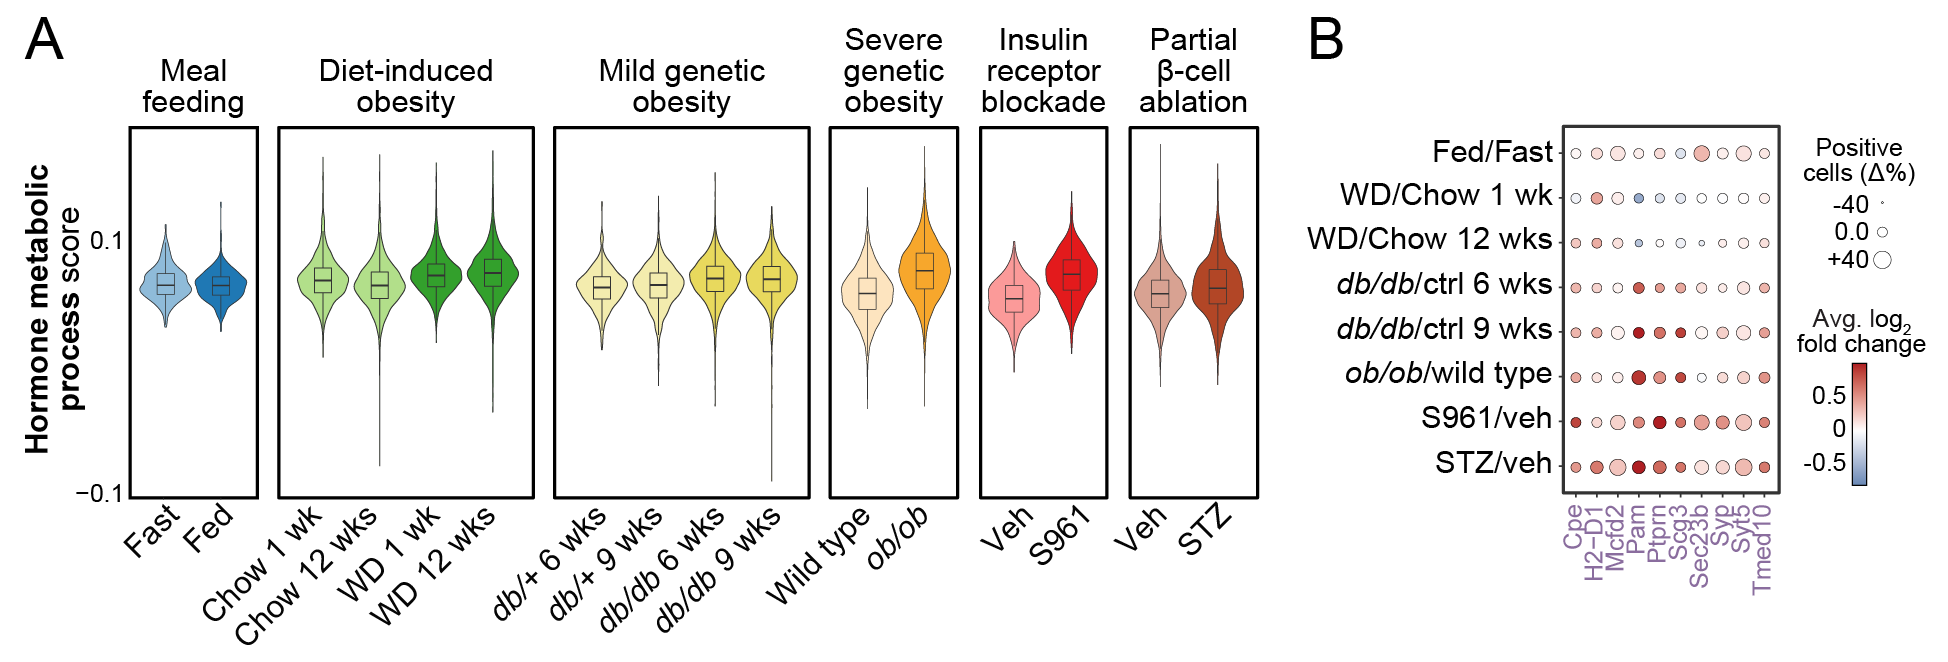
\includegraphics[width=\linewidth]{Chapter5/Fig/F3-13-02.png}
\caption[Gene-set scoring of `\textit{Hormone metabolic process}']{\textbf{Activity of genes associated with Hormone metabolic process.} \textbf{(A)} Violin plots depicting the gene-set score for `Hormone metabolic process' associated genes shown for β-cell workload models and corresponding healthy controls from individual studies. On the overlay boxplots, the middle horizontal line represents the median, the box represents the inter-quartile range and the whiskers represent the minimum and maximum values. The number of cells are indicated in Supplementary Table \ref{tab:3-3}. \textbf{(B)} Differential expression of few of the `Hormone metabolic process' associated genes across β-cell workload models compared to their respective controls. The color and size of the dots represent the average log fold change of expression and the difference in percentage of cells between the models and their respective controls.}
\label{fig:3-13-2}
\end{figure}


\subsubsection{Ribosome biogenesis}
Ribosomes are cellular factories that make proteins. Following a similar expression profile to `Hormone Metabolism', the feeding intervention and WD-induced obesity did not result in a higher score for genes related to `Ribosome biogenesis'. While only a few genes in this gene set showed weaker upregulation, several genes were downregulated in response to these models. This echoes a similar observation of reduced expression of several ribosome biogenesis genes in a \gls{hfd} model. \textbf{\cite{https://www.nature.com/articles/s41598-017-03869-5}}. Conversely, this gene set was upregulated in both models of genetic obesity (\textit{db/db} and \textit{ob/ob}) and following S961- and \gls{stz}-treatment. A significant increase in the expression of ribosome-related molecules has been demonstarted in islets isolated from \textit{db/db} mice \textbf{\cite{https://pubmed.ncbi.nlm.nih.gov/19309774/}}. The strong upregulation of ribosomal markers in the \textit{ob/ob} mice and following S961-treatment could be attributed as an response to the hyperglycemic environment leading to compensatory, increased insulin production and this effect is amplified in case of \gls{stz}-treatment, where the surviving population of β-cells following ablation are unable to prevent hyperglycemia. The upregulation of the ribosomal markers in the three hyperglycemic models was also consistent with the expression of ribosomal protein genes correlating with loss of β-cell maturity along the the Maturity (PC1) axis.

\begin{figure}[H]
\centering
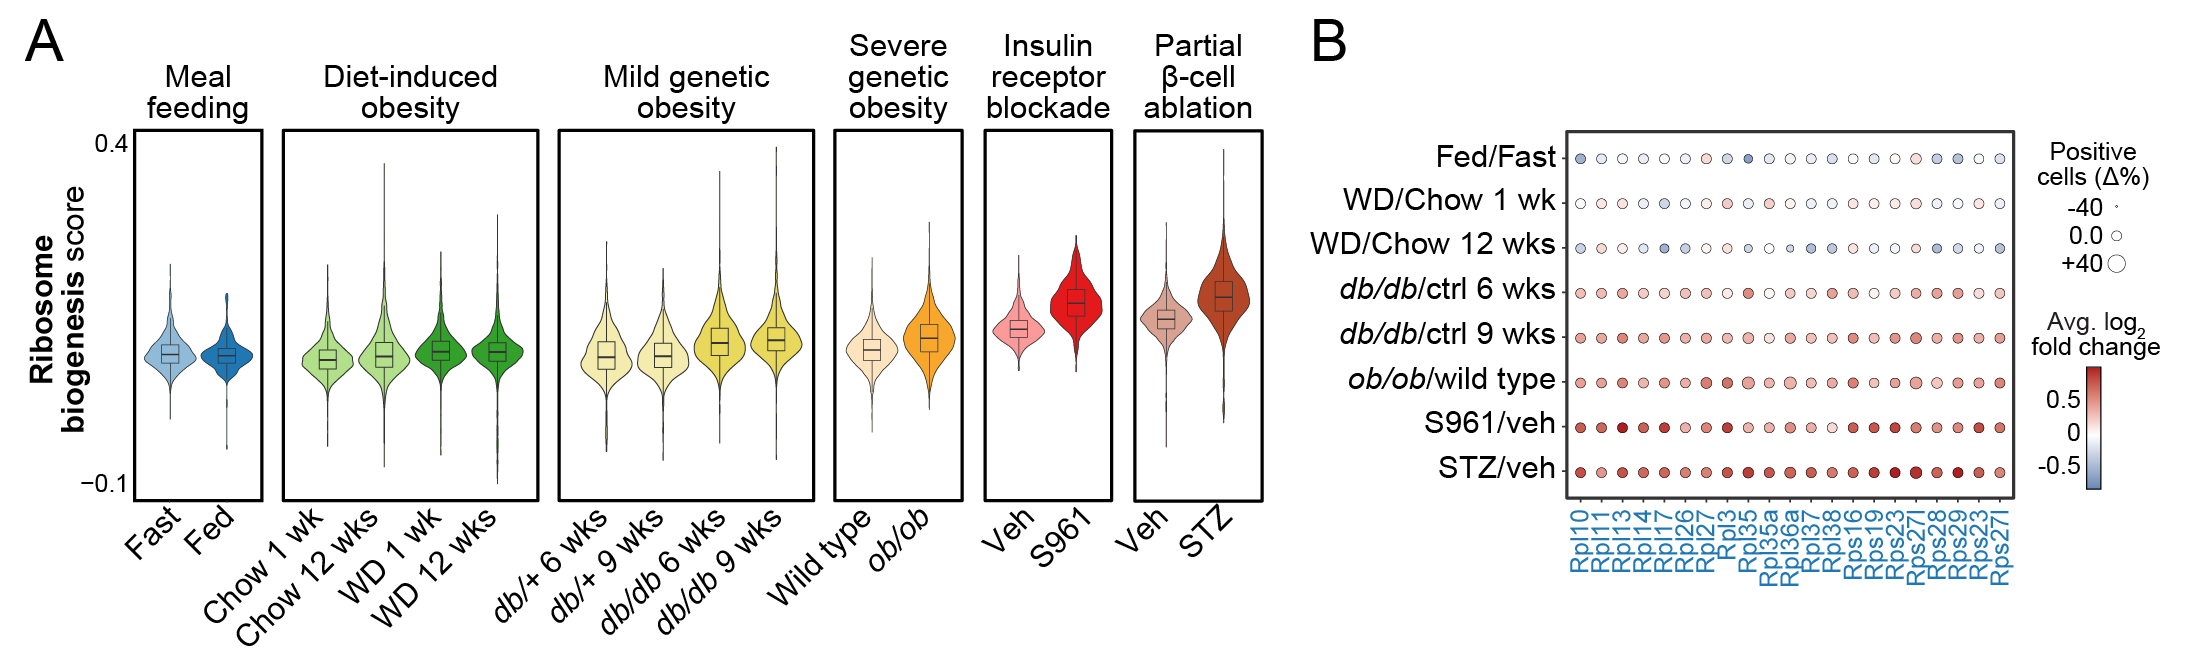
\includegraphics[width=\linewidth]{Chapter5/Fig/F3-13-03.png}
\caption[Gene-set scoring of `\textit{Ribosome biogenesis}']{\textbf{Activity of genes associated with Ribosome biogenesis.} \textbf{(A)} Violin plots depicting the gene-set score for `Ribosome biogenesis' associated genes shown for β-cell workload models and corresponding healthy controls from individual studies. On the overlay boxplots, the middle horizontal line represents the median, the box represents the inter-quartile range and the whiskers represent the minimum and maximum values. The number of cells are indicated in Supplementary Table \ref{tab:3-3}. \textbf{(B)} Differential expression of few of the `Ribosome biogenesis' associated genes across β-cell workload models compared to their respective controls. The color and size of the dots represent the average log fold change of expression and the difference in percentage of cells between the models and their respective controls.}
\label{fig:3-13-3}
\end{figure}


\subsubsection{Proteasomal Catabolic process}
The gene-set `Proteasomal Catabolic process' was upregulated in all models of increasing β-cell workload. The genes comprising this gene-set were canonical unfolded protein response (UPR) and endoplasmic reticulum (ER)-associated protein degradation (ERAD) markers. The UPR is a critical adaptive response to ER stress, restoring cell homeostasis and contributing to loss of β-cell mass in T2D \textbf{\cite{oppenlander_vertical_2021,fonseca_endoplasmic_2011,bilekova_pharmacological_2021}}. UPR genes such as \textit{Hspa5, Edem2, Derl3} and \textit{Herpud1} were found to be upregulated on the mRNA level in response to various models of increasing β-cell workload. The ERAD pathway serves to mitigate ER stress and has been attributed an indispensable role in the maintenance of β-cell identity and function \textbf{\cite{oppenlander_vertical_2021,hu_endoplasmic_2019,shrestha_sel1l-hrd1_2020}}. The expression of ERAD genes such as \textit{Derl3, Dnajb9, Edem1/2, Herpud1, Hspa5, Hsp90b1, Sec61b, Selenos} were also upregulated in all studies. Therefore, increases in β-cell workload enhances adaptive-response mechanisms to ER stress in β-cells in response to \hl{...}

\begin{figure}[H]
\centering
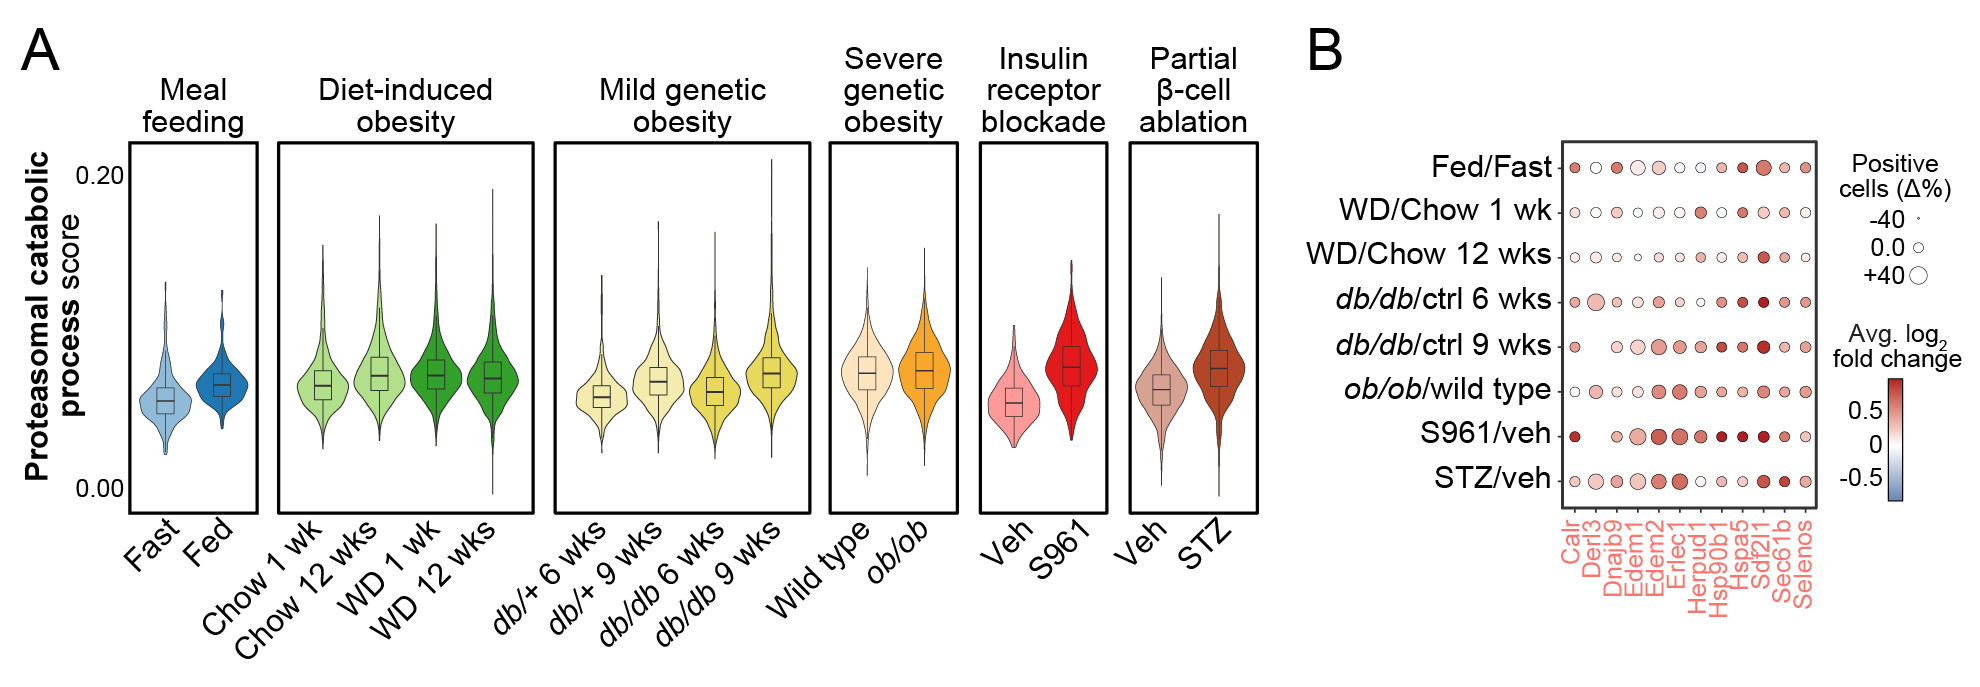
\includegraphics[width=\linewidth]{Chapter5/Fig/F3-13-04.png}
\caption[Gene-set scoring of `\textit{Proteasomal catabolic process}']{\textbf{Activity of genes associated with Proteasomal catabolic process.} \textbf{(A)} Violin plots depicting the gene-set score for `Proteasomal catabolic process' associated genes shown for β-cell workload models and corresponding healthy controls from individual studies. On the overlay boxplots, the middle horizontal line represents the median, the box represents the inter-quartile range and the whiskers represent the minimum and maximum values. The number of cells are indicated in Supplementary Table \ref{tab:3-3}. \textbf{(B)} Differential expression of few of the `Proteasomal catabolic process' associated genes across β-cell workload models compared to their respective controls. The color and size of the dots represent the average log fold change of expression and the difference in percentage of cells between the models and their respective controls.}
\label{fig:3-13-4}
\end{figure}


\subsubsection{Transport Vesicle}
Diet models such as the feeding intervention and diet-induced obesity exhibited opposite patterns for the ‘transport vesicle’ gene set.  Feeding intervention resulted in minor upregulation of the gene set (exemplary genes did not show a high magnitude of fold-change) whereas diet-induced obesity after 1 or 12-weeks of feeding depicted that this gene set was rather downregulated (even though some of the genes were upregulated by a higher magnitude than feeding intervention). This could be explained by an acute increase in transport vesicle dynamics upon feeding compared to chronic effects of obesity leading to eventual β-cell dysfunction and therefore the downregulation of these processes. Genetic pre-disposition to diabetes via the db/db and ob/ob models also exhibited an upregulation of the vesicle gene-set, although the magnitude in the  \textit{ob/ob} model was lower. The treatment-induced hyperglycemic models such as S961-treatment and \gls{stz}-treatment were strongly associated with changes in transport vesicle (\textit{Atp1a1, Stub1}). This strong upregulation could be a result of activation of responses to cellular stress as way for β-cells to maintain function by increasing the expression of genes.\\

% \begin{figure}[t]
% \centering
% 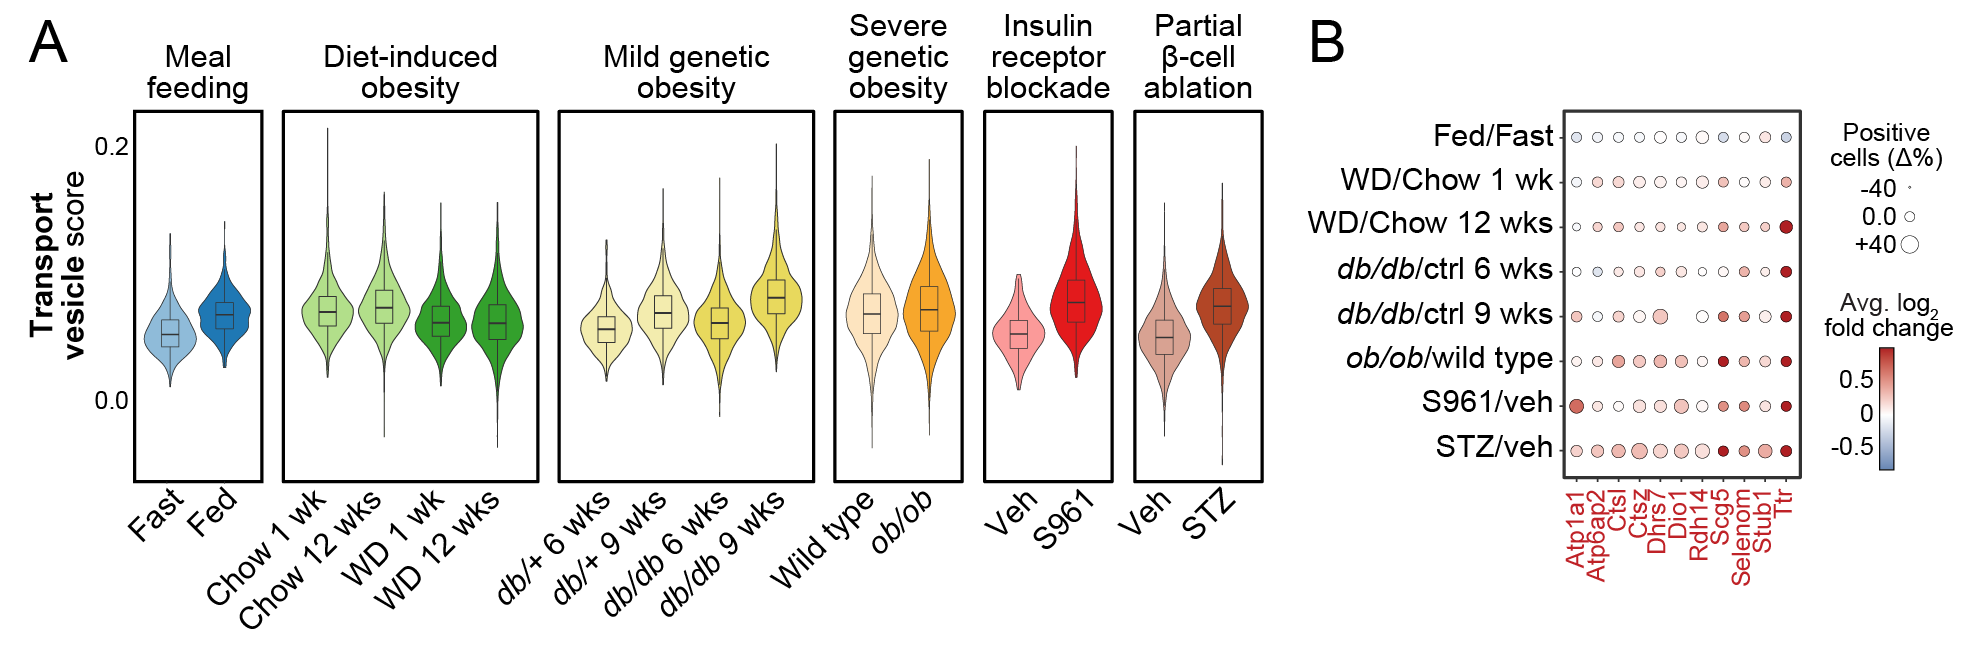
\includegraphics[width=\linewidth]{Chapter5/Fig/F3-13-05.png}
% \caption[Gene-set scoring of `\textit{Transport vesicle}']{\textbf{Activity of genes associated with Transport vesicle across studies.} \textbf{(A)} Violin plots depicting the gene-set score for `Transport vesicle' associated genes shown for β-cell workload models and corresponding healthy controls from individual studies. On the overlay boxplots, the middle horizontal line represents the median, the box represents the inter-quartile range and the whiskers represent the minimum and maximum values. The number of cells are indicated in Supplementary Table \ref{tab:3-3}. \textbf{(B)} Differential expression of few of the `Transport-vesicle' associated genes across β-cell workload models compared to their respective controls. The color and size of the dots represent the average log fold change of expression and the difference in percentage of cells between the models and their respective controls.}
% \label{fig:3-13-5}
% \end{figure}


In summary, β-cell compensatory responses to heightened demands of increased workload resulted in overall downregulation of markers related to β-cell identity and function, and induced pathways related to ER and metabolic stress,  and upregulated cellular machinery related to ribosomal biogenesis and  vesicle trafficking. Further, this analysis served as extension to the MIA by recapitulating the findings of similarity between human T2D and mouse models of β-cell dysfunction in the context of diet and feeding induced stress, severe genetic obesity and insulin receptor blockade by S961-treatment. 

\clearpage

\section{Reference learning}
\label{sec:chp3_validation}

%A major advantage of single-cell atlases is the ability to learn and transfer the findings from a reference study onto an external query dataset. This is particularly useful in cases of cell-type or state transfer between two or more studies as well as for comprehensive comparisons across several studies and/or conditions. Reciprocally, the atlases can benefit from transfer learning as it enhances the utility and applicability of these resources. The mapping of wide-variety of single-cell datasets exploring various aspects of development, health and disease onto references ultimately extends the scope of the atlases, thereby allowing for further refinement of cell-type annotation, improved data integration and robustness to data variability and facilitating discovery of novel biological insights.

The capacity to learn and apply the results from a reference study onto an external query dataset is a significant benefit of single-cell atlases. This is especially helpful for thorough comparisons across multiple studies and/or conditions, as well as for cell-type or state transfer between two or more studies. Reciprocally, the atlases can benefit from transfer learning as it enhances the utility and applicability of these resources. The mapping of wide-variety of single-cell datasets exploring various aspects of development, health and disease onto references ultimately extends the scope of the atlases, thereby allowing for further refinement of cell-type annotation, improved data integration and robustness to data variability and facilitating discovery of novel biological insights.\\

To demonstrate the usefulness of the integrated β-cell transcriptome generated in this analysis, we mapped two additional mouse datasets onto this reference. These datasets are not included in the integrated atlas of β-cell workload models. Instead they were projected onto the reference to transfer annotations from the reference to  queries. Both datasets were generated using the 10x scRNA-seq workflow and the raw data was re-processed using a pipeline similar to that used for sample processing and quality control in the integrated atlas. This ensured that technical batch effects didn't influence the subsequent mapping steps. One of the studies used in this validation analysis was an in-house generated dataset of islets from lean mice and obese, insulin resistant \textit{db/db} mice, with β-cell specific knockout of lysine-specific histone demethylase 1 (\textit{Lsd1}), which restrains the adaptive insulin secretion of β-cells in response to feeding \textbf{\cite{wortham_nutrient_2023}}. The other study was a previously published dataset of islets from mice subjected to a high-fat diet (HFD) induced glucose intolerance \textbf{\cite{fu_single-cell_2023}}.

\subsection{Mapping with \textit{db/db}-\textit{Lsd1} study}

In a recent study, Wortham \textit{et al.} elucidated the nuanced regulation of β cell functional adaptation by the epigenome whereby nutrient availability modules β cell responses through histone hyperacetylation and transcription. Central to this regulation is chromatin modifying lysine-specific histone demethylase 1 (\textit{Lsd1}) that acts as a dynamic regulator of chromatin accessibility in response to acute changes in nutrient state during feeding and fasting cycles. Interestingly, in an insulin-resistant model of chronic β-cell adaptation (\textit{db/db}), the analysis also found overlap with genes upregulated in acute β cell response to feeding along with hyperacetylation at many of the feeding-induced sites. Additionally, \textit{Lsd1}-bound active chromatin was also enriched for T2D-associated risk variants, suggesting that T2D risk variants can influence the activity of the \textit{Lsd1}-regulated network. Thus, these findings support a model whereby the β-cell adaptation of insulin secretory response is regulated at the level of the epigenome, with influences from environmental nutrient signals and genetic variation \textbf{\cite{wortham_nutrient_2023,aamodt_peeling_2023}}.\\

%unveiled the islet epigenome as a pivotal regulatory layer in the β-cell functional adaptation to changes in insulin demand. Through integrated studies of β cell physiology, epigenomics, and transcriptomics \\

%To further understand why β-cells fail in \textit{Lsd1} knockout obese \textit{db/db} mice, 
To dissect the role of \textit{Lsd1} in β-cell compensatory mechanisms during insulin resistance, scRNA-seq was performed on islets prior to and after the onset of glucose intolerance. The homozygous (\textit{db/db}) obese animals and their corresponding heterozygous (\textit{db/+}) lean mice were crossed with \textit{Lsd1\textsuperscript{fl/fl}} mice, in order to conditionally knockout \textit{Lsd1}, specifically in β-cells. This resulted in the following four experimental cohorts:
\begin{itemize}
    \item Control (\textit{db/+ Lsd1\textsuperscript{fl/+β}})
    \item Lean mice with \textit{Lsd1} knockout (\textit{db/+ Lsd1\textsuperscript{$\Delta$β}})
    \item Obese mice with \textit{Lsd1} intact (\textit{db/db Lsd1\textsuperscript{fl/+β}}) and
    \item Obese mice with \textit{Lsd1} knockout (\textit{db/db Lsd1\textsuperscript{$\Delta$β}})
\end{itemize}


To identify functional processes that are characteristic of the β-cells obtained from the islets of lean and obese mice with or without \textit{Lsd1} knocked-out, we performed gene-set scoring of the modules identified from the hierarchical clustering analysis of pseudo-bulk β-cells across all samples (\textit{see} Section \ref{sec:chp3_pseudobulk}). As expected, the `Workload-repressed' module was upregulated in lean mice with \textit{Lsd1} intact. This module consisted of developmental-identity and functional-identity genes. This was also observed in case of the older animals, wherein the module was further upregulated compared to the younger 6 week old mice. Further, the activity of this module progressively declined in lean mice when \textit{Lsd1} was deleted, followed by obese animals with \textit{Lsd1} intact and \textit{Lsd1} deletion, in which the genes were least active. Interestingly, the 9-week-old obese mice with \textit{Lsd1} deleted strongly associated with this module in-comparison to their 6-weeks old counterparts. This could likely be due to the additive nature of \textit{db/db} and \textit{Lsd1} effects, which work to enhance insulin secretion, resulting in upregulation of secretion machinery, but at the cost of later defects.